\documentclass[12pt]{book}
\usepackage[hideStatements]{omi2}
\usepackage[paperheight=9in,paperwidth=6.75in,left=1in]{geometry}
\begin{document}	
	
\title{Olimpiada de Informática}
\author{---}
\date{---}
\setcounter{tocdepth}{1}
\frontmatter

\maketitle
\tableofcontents

\mainmatter

\part{Elementos básicos}

\part{Búsquedas}
\chapter[Búsqueda Exhaustiva]{Búsqueda exhaustiva\\ Fuerza bruta}
Muchas veces en nuestra vida hemos tenido que buscar algo, una foto en nuestra galería del teléfono, una palabra en el diccionario, una carta dentro de un mazo, etc. Y probablemente, con la experiencia, hemos aprendido algunas intuiciones sobre como buscar cosas, en esta parte trabajaremos un poco más en desarrollar esta intuición e ideas.

En la olimpiada de informática también debemos buscar cosas. Ya sea encontrar la solución al problema o solo utilizar una búsqueda como paso intermedio, ser buenos haciendo búsquedas nos abrirá la puerta a muchos problemas y técnicas.

Para comenzar con entendiendo las búsquedas comenzaremos con la búsqueda más sencilla, la búsqueda exhaustiva, también conocida como fuerza bruta. 

Lo primero que se requiere para poder buscar es definir el espacio de búsqueda, ¿dónde podría estar lo que queremos encontrar? De la respuesta dependerá como haremos la búsqueda. Por ejemplo, si buscamos la posición de un valor en un arreglo, el espacio de búsqueda es el arreglo.

Una vez que definamos donde podría estar la respuesta, lo que hacemos con la exhaustiva es explorar absolutamente todo el espacio de búsqueda, todos los candidatos que podrían ser lo que buscamos hasta dar con la respuesta. Por esto se le conoce como fuerza bruta, porque aprovecha el poder computacional para procesar todo hasta dar con la respuesta.

Se te enseñara las búsquedas exhaustivas más comunes, así como una forma general. En concreto, los espacios de búsquedas que usaremos son:

\begin{plimits}
	\item Espacio lineal
	\item Parejas de elementos
	\item Ordenes (Permutaciones)
	\item Subcojuntos
\end{plimits}
 
 Y terminaremos este capitulo aprendiendo como hacer búsqueda exhaustiva de forma general usando recursión e iteración.
 

 



\section{Búsqueda lineal}
\markright{BÚSQUEDA LINEAL}
La búsqueda lineal es la más sencilla de las búsquedas que hay. ¿Qué es lo que harías si te pido que de una pila de exámenes encuentres el tuyo? Lo que probablemente hagas es una revisar uno por uno, checar de arriba hacia abajo hasta que encuentres el examen con tu nombre en él.

Básicamente, esta idea es la búsqueda lineal, ir revisando de uno por uno toda una lista de candidatos hasta encontrar al que estas buscando o hasta que hayas revisado todos los candidatos.

Entonces, los códigos de búsqueda lineal casi siempre tendrán la siguiente estructura:

\begin{lstlisting}
	Itera por cada candidato {
		Si el candidato es lo que buscamos {
			Respuesta = candidato;
			Detener ciclo /* esto es opcional, depende si hay varios valores que queramos encontrar. */
		}
	}	
\end{lstlisting}

Veamos cómo usar esta técnica para resolver un problema.

\subsection*{Ejemplo: Encontrar posición en un arreglo}

Supongamos que queremos tenemos un arreglo \(A\) de enteros distintos y este tiene \(N\) elementos en él. Nosotros querremos hacer un código que imprima la posición del arreglo que valga \(K\). O si este valor no existe, que imprima \(-1\).

\subsection*{Límites}
\begin{plimits}
	\item \(1\leq N \leq 10^5\)
	\item \(1\leq K,A[i] \leq 10^9\)
\end{plimits}

ENLACE: TODO

\subsection*{Solución}

(Recuerda intentar el problema antes de leer la solución)

Lo que este problema nos pide en realidad es buscar dentro del arreglo por el índice del elemento \(K\).

Lo que haremos es revisar todas las posiciones del arreglo hasta encontrar aquella que valga \(K\), si no la encontramos imprimimos \(-1\).


\subsection*{Código}
\begin{lstlisting}
	int A[100050];
	int N, K;
	int main () {	
		ios_base::sync_with_stdio(0); cin.tie(0);
		cin >> N;
		for (int  i=0; i <N; i++){ 
			cin >> A[i];
		}
		cin >> K;
		int respuesta = -1;
		for (int i =0; i < N; i++) {
			if (A[i]==K) {
				respuesta = i;
				break;
			}
		}
		cout << respuesta;
	}
\end{lstlisting}


\subsection{Complejidad}

Una pregunta que te has de hacer es: ¿cuál es la complejidad de esta técnica? Y la respuesta es sencilla, en el peor de los casos tenemos que revisar a todos los candidatos, digamos que la cantidad de ellos es iguala a \(N\), entonces la complejidad es \(O(N)\).

\subsection*{Ejemplo: Contar formas de dividir}
Veamos otro problema de búsqueda lineal. 

\subsection*{Descripción}

Carlos quiere armar una fiesta, y como le gusta ser un buen anfitrión compro \(N\) regalos para sus invitados.
Ahora, Carlos quiere darle la misma cantidad de regalos a cada uno de sus invitados sin que sobre ningún regalo no repartido. Como Carlos le gusta contar, ahora se pregunta: ¿Cuántas cantidades diferentes de invitados puede tener?
\subsection*{Entrada}
Un entero \(N\), indicando cuantos regalos compró Carlos.
\subsection*{Salida}
La cantidad de posibles números de invitados para la fiesta.
\subsection*{Casos ejemplo}
\begin{casebox2}
	\scase{12}{6}
	\scase{7}{1}
	\scase{4}{3}
\end{casebox2}
\subsection*{Límites}
\begin{plimits}
	\item \(1\leq N \leq 10^5\)
\end{plimits}

\subsection*{Solución}
Es fácil ver que el problema en realidad pregunta: ¿Cuántos divisores positivos tiene \(N\)?

(Nota: un divisor de \(N\) es un número que divide a \(N\) sin decimales).

Encontremos todos los divisores de \(N\). Estos se encontrarán entre \(1\) y \(N\), por lo que podemos iterar i por todo este rango revisando si \(i\) es divisor de \(N\).
\subsection*{Código}
\begin{lstlisting}
	respuesta = 0;
	for (int i =1; i <= N; i++) {
		if (N%i==0) {
			respuesta++;
		}
	}
	cout << respuesta;
\end{lstlisting}

\section*{Problemas de practica}
\addcontentsline{toc}{section}{Problemas de práctica}

\begin{exercise}
	\problema[problemas/frecuencia-de-k]{TODO Frecuencia de K}{\omegauplink{frecuencia-de-k}}
\end{exercise}

\begin{exercise}
	\problema[problemas/multiplos-de-cinco]{TODO Multiplos de cinco}{\omegauplink{multiplos-cinco}}
\end{exercise}

\begin{exercise}
	\problema[problemas/divisores]{TODO: Divisores del entero}{\omegauplink{divisores-entero}}
\end{exercise}

\begin{exercise}
	\problema[problemas/suma-de-digitos]{A la suma de digitos}{\omegauplink{m-suma-digitos}}
\end{exercise}

\begin{exercise}
	\problema[problemas/escalera-de-fer]{Escalera de fer}{\omegauplink{}}
\end{exercise}



\section{Búsqueda lineal con función de validación}
\markright{BÚSQUEDA LINEAL CON FUNCIÓN DE VALIDACIÓN}

Hasta ahorita hemos visto problemas donde revisar si un candidato era la respuesta o no bastaba con un simple condicional, pero este no siempre es el caso.

Varías veces, para revisar si un valor es solución a nuestro problema, vamos a tener que necesitar un poco más de código e ideas. Veamos un problema de este estilo.

\subsection{Ejemplo: Dividiendo listones}


\subsection*{Descripción}
Karel tiene \(N\) listones de distintas longitudes enteras. Karel quiere hacer pulseras con ellos, por lo que tomará cada uno de los listones y los cortará para que las pulseras usen segmentos del mismo tamaño.

A Karel le gustan los enteros, entonces la longitud de los segmentos también ha de serla. Además, Karel no quiere que sobre listón sin usar ¿Cuántos diferentes tamaños de segmento se pueden elegir?

\subsection*{Entrada}
Un entero \(N\), indicando la cantidad de listones
En la siguiente línea, \(N\) enteros indicando las longitudes de los listones. Llamemos \(A[i]\) a la longitud del listón \(i\).

\subsection*{Salida}
La cantidad de opciones para el tamaño de los segmentos

\subsection*{Caso ejemplo}
\begin{casebox3}
	\ecase{
		5 \\ 
		10 30 20}
	{3}
	{Las longitudes pueden ser 1, 2 y 5}
\end{casebox3}	
\subsection*{Límites}
\begin{plimits}
	\item \(1\leq N \leq 100\)
	\item \(1\leq A[i] \leq 5000\)
\end{plimits}

\subsection*{Código}
Encontremos con búsqueda lineal todos los tamaños de segmento que cumplen y contemos cuantos son.

Primero veamos que los tamaños de listón deben estar entre 1 y 5000. Más concreto, entre \(1\) y \(min (A[1],A[2],\cdots ,A[N])\). Esto es porque el tamaño del segmento debe ser entero, debe ser por lo menos 1 (ya que un segmento de tamaño 0 o menor no tiene sentido para este problema) y no puede ser más largo que el listón más corto.

Ya hemos visto como se ve una búsqueda lineal y la que usaremos en este caso sería:

\begin{lstlisting}
	cin >> N;
	for (int i=0; i< N; i++) {
		cin >> A[i];
	}
	
	int minA=A[0];
	for (int i=1; i < N; i++) {
		minA=min(minA, A[i]); /* encuentra el liston mas
		pequeno. */
	}
	respuesta = 0;
	for (int s =1; s <= minA; s++) {
		if (es s es un tamano de segmento valido) {
			respuesta++;
		}
	}
	cout << respuesta
	
\end{lstlisting}

Pero el reto ahora es el chequeo de “es s es un segmento de tamaño valido”.

Para esto necesitamos un poco más de trabajo. Veamos un solo listón. Si queremos cortarlo en segmentos de tamaño s sin que sobre, ¿qué tiene que cumplir s con relación al listón? Así es, que es, que s divida a la longitud del listón. Y podemos ver que s tiene que cumplir esto para todos los listones

Entonces, para ver que s sea una opción válida, hay que ver que s divida a todos los enteros en la lista de listones.

Para lograr esto, creemos una función booleana que se encargue de validar s.
\begin{lstlisting}
	bool validar (int s) {
		bool respuesta = true;
		for (int i=0; i< N; i++) {
			if (A[i]%s!=0){
				respuesta = false;
				break;
			}
		}
		return respuesta;
	}
\end{lstlisting}

Entonces con esta función obtenemos que el código de la búsqueda lineal ahora es:
\begin{lstlisting}
	respuesta = 0;
	for (int s =1; s <= minA; s++) {
		if (validar(s)) {
			respuesta++;
		}
	}
	cout << respuesta
	
\end{lstlisting}

Y con esto logramos completar el problema.

\subsection{Complejidad}
La búsqueda lineal la hacemos sobre el valor de A, pero, además, por cada iteración de la búsqueda lineal, hacemos un ciclo que revisa la condición para que s sea contada.

Entonces, la complejidad nos queda como:   \(O(Busqueda\times Validar)=O(AN)\).

Como \(A\leq 5000\) y \(N\leq 100\). Nos queda que \(AN\leq 5\times 10^5\), lo cual corre en menos de un segundo.


\section*{Problemas de práctica}
\addcontentsline{toc}{section}{Problemas de práctica}


\begin{exercise}
	\problema[problemas/bicicleta-de-karel]{Bicicleta de Karel I}{\omegauplink{bicicleta-de-karel-i}}
\end{exercise}

\begin{exercise}
	\problema[problemas/contar-capicuas]{Contar capicúas}{\omegauplink{Contar-capicuas}}
\end{exercise}

\begin{exercise}
	\problema[problemas/cuenta-primos]{Cuenta primos}{\omegauplink{Cuenta-primos}}
\end{exercise}

\section{Parejas de elementos}

\markright{PAREJAS DE ELEMENTOS}

En muchos problemas nos pedirán que encontremos o contemos la cantidad de pares que cumplan alguna condición, o nosotros convertiremos a un problema de este estilo. Para este tipo de problemas será útil conocer como hacer una búsqueda completa que revise todas las posibles parejas de elementos.

Como antes, veamos un problema que puede ser resuelto con esto.

\subsection*{Ejemplo: Pares de suma K}

Fernando necesita \(K\) tornillos de la ferretería. Sin embargo, la vida no siempre es fácil y la ferretería no vende exactamente \(K\) tornillos.

Sin embargo, venden \(N\) cajas de tornillos cada una con \(C_i\) tornillos dentro. 

Como Fernando tiene una obsesión con no desperdiciar, él solo comprara las cajas de forma que traigan juntas exactamente \(K\) tornillos. Además, odia las bolsas de un solo uso que dan en la ferretería por lo que solo comprará dos cajas, una por cada mano.

Entonces, dado el tamaño de las cajas, determina si Fernando puede traer consigo exactamente \(K\) tornillos.

\subsection*{Entrada}
Dos enteros, \(N\) y \(K\), representando cuantas cajas hay y cuantos tornillos se requieren.

En la siguiente línea vendrán \(N\) enteros separados por espacios, indicando la cantidad de tornillos en cada caja.

\subsection*{Salida}
Deberás imprimir “SI” en caso de que Fernando pueda obtener K tornillos con sus reglas, o “NO” si es imposible.

\subsection*{Casos ejemplo}

\begin{casebox3}
	\ecase{
		4 6 \\
		3 1 8 5
	}
	{SI}
	{Usa las cajas con 1 y 5 tornillos.}
	\ecase{
		5 10\\
		3 1 8 5 12
	}
	{NO}
	{}
\end{casebox3}

\subsection*{Límites}
\begin{plimits}
	\item \(1\leq N \leq 1000\)
	\item \(1\leq K \leq 10^9\)
	\item \(1\leq C_i \leq 10^9\)
	\item \(C_i \neq K\)
\end{plimits}

Enlace: [TODO]

\section * {Solución}

Lo que nos pregunta el problema es: ¿Existe un par de cajas tal qué sumen \(K\)?

Para determinar si existe dicha pareja, lo que haremos será buscar entre todas las parejas de cajas aquella que sume \(K\). Es decir, buscaremos completamente todas las parejas posibles.

Para iterar por todas las parejas lo que haremos es primero definir una pareja como dos índices \((i,j)\), tal que \(0\leq i < j <N\).  Como queremos iterar por todos los posibles pares, primero iteraremos por todos los valores de \(i\). Y para cada \(i\), iteraremos por todas las \(j\) con las que se puede emparejar. El código se ve como:

\begin{lstlisting}
	for (int i =0; i < N; i++) {
		for (int j=i+1; j< N; j++) {
			cout << i<<" "<<j<< "\n";/* imprimimos 
			cada par */ 
		}
	}
\end{lstlisting}

Y ahora que sabemos iterar por todos los pares, lo utilizamos para revisar si existe un par que sume \(K\). 

\begin{lstlisting}
	for (int i =0; i < N; i++) {
		for (int j=i+1; j< N; j++) {
			if (Caja[i]+Caja[j] == K) {
				cout << "SI";
				exit(0); /* Termina el programa, 
				encontramos la respuesta */
			}
		}
	}
	cout << "NO";
\end{lstlisting}

Entonces, son estos dos ciclos for nos permiten iterar por toda pareja de elementos en un arreglo. Esta es una herramienta bastante útil para resolver muchos problemas y subtareas.

\subsection {Complejidad}
Bien, ahora hablemos de la complejidad de esta técnica. La complejidad es \(O(N^2)\). Esto es porque la cantidad de parejas con \(N\) elementos crece en\(O(N^2)\).

Pero incluso si no conocemos como crecen las parejas, podemos ver que este ciclo para \(i = 0\), itera por \(N-1\) valores de \(j\); para \(i=1\), iteramos por \(N-2\) valores de \(j\); para \(i=2\), iteramos por \(N-3\) valores de \(j\), y así sucesivamente. De forma que hacemos \((N-1)+(N-2)+\ldots+1+0\) iteraciones de \(j\). Entonces hacemos \(1+2+3+\ldots+(N-1)\) iteraciones.

Usando la formula se suma de gauss\footnote{Formula de gauss para sumar los primeros \(N\) naturales: \(1+2+3+\ldots+N=\frac{N(N+1)}{2}\)} obtenemos que:

\[1+2+3+\ldots+(N-1)=\frac{N(N-1)}{2}=\frac{N^2}{2}-\frac{N}{2}\]

Entonces, la complejidad queda como \(O(\frac{N^2}{2}-\frac{N}{2})=O(N^2)\)

Por lo tanto, iterar por todos los pares de un arreglo es una técnica de complejidad cuadrada, perfecta para límites hasta \(\sim{10^4}\).

\begin{exercise}
	Una inversión en un arreglo es una pareja de números \(i\) y \(j\) que cumplen: \(i < j\) y \(A[i] > A[j]\), es decir, estos dos números están desordenados con relación entre ellos.
	
	Dado un arreglo de \(N\) enteros, determina cuantas inversiones tiene. (\(1\leq N \leq 1000\)).
	
	(TODO)
\end{exercise}

\begin{exercise}
	Búsqueda lineal encuentra un solo elemento, aquí aprendimos a buscar una pareja, dos elementos. Crea el código para buscar una tercia de elementos en un arreglo que sume \(K\).
		
	No olvides analizar la complejidad.\\
	(TODO).
\end{exercise}



\section{Ordenes o permutaciones}
\markright{ORDENES O PERMUTACIONES}

En algunos problemas nos pedirán que encontremos un ordenamiento.

TODO HACER ESTO
\section{Subconjuntos}
\markright{SUBCONJUNTOS}

\subsection{Conjuntos y subconjuntos}

Un conjunto no es nada mas que una colección de objetos. Por ejemplo, si alguien trae en su mochila un plátano, manzana y naranja, este puede decir que trae un conjunto de frutas compuesto por un plátano, manzana y naranja.

En matemáticas e informática, nosotros estamos trabajando todo el rato con los conjuntos. Ya sean el conjunto de datos de entrada, o los números enteros, tener noción de conjuntos es un requerimiento para el éxito en la olimpiada.

Veamos un poco de notación. Para escribir el conjunto A de números esta conformado por el 3, 5 y 9 escribimos lo siguiente:
\[A=\{3,5,9\}\]

\begin{center}
	\textbf{TODO: CORREGIR ESTO}
\end{center}
\pagebreak

\subsection{Ejemplo: Enlistar subconjuntos}
Veamos como hacer para visitar todos los subconjuntos, lo cuál será necesario para problemas donde nos preguntan por ellos.

Para esto, primero aprendamos a resolver el problema que trata de mostrar los subconjuntos:

\subsection*{Problema:}

Karel tiene un conjunto formado por las primeras \(N\) letras del alfabeto. Ahora Karel que imprimas todos los subconjuntos, uno por cada línea. Puedes imprimirlos en cualquier orden.

Cada subconjunto es representado por las letras en el de la A a la Z. El subconjunto vacío será representado por un asterisco '*'.
\subsection*{Entrada}
Un entero \(N\), indicando cuantas letras hay en el conjunto.
\subsection*{Salida}
Todos los subconjuntos

\subsection*{Ejemplos}

\begin{casebox2}
	
	\scase{2}{
		AB\\
		A \\
		B\\
		*
	}
	\hline
\end{casebox2}

\begin{casebox2}
	\scase{3}
	{
		ABC \\
		AB \\
		AC\\
		A\\
		BC\\
		B\\
		C\\
		* \\
	}
	\hline
\end{casebox2}

\subsection*{Límites}
\begin{plimits}
	\item \(1\leq N \leq 20 \)
\end{plimits}

\subsection*{Solución}

Entonces, podemos resolver el problema si obtenemos todos los subconjuntos posibles. Para esto, haremos un algoritmo que construya todos los posibles subconjuntos.

Esto se puede hacer de dos formas principales, una iterativa y otra recursiva. Comencemos viendo la forma con recursión.

\subsection* {Subconjuntos usando recursión}

Digamos que \(S(conjunto)\) sean todos los subconjuntos del \(conjunto\). Por ejemplo:
\[S(\{A,B,C\})=\]
\[\{\{A,B,C\},\{A,B\},	\{A,C\},\{A\},\{B,C\},	\{B\},\{C\},	\emptyset\} \]

O usando la misma notación que la salida del problema (la que usaremos a partir de aquí):

\[S(ABC)=\{ABC, AB, AC, A, BC, B, C, * \}\]

Veamos un poco como se comporta S, por ejemplo para \(N = 4\), en total tenemos 16 subconjuntos los cuales podemos dividir en dos mitades con 8 cada una, los que tienen la A y los que no tienen la A.



\begin{center}
	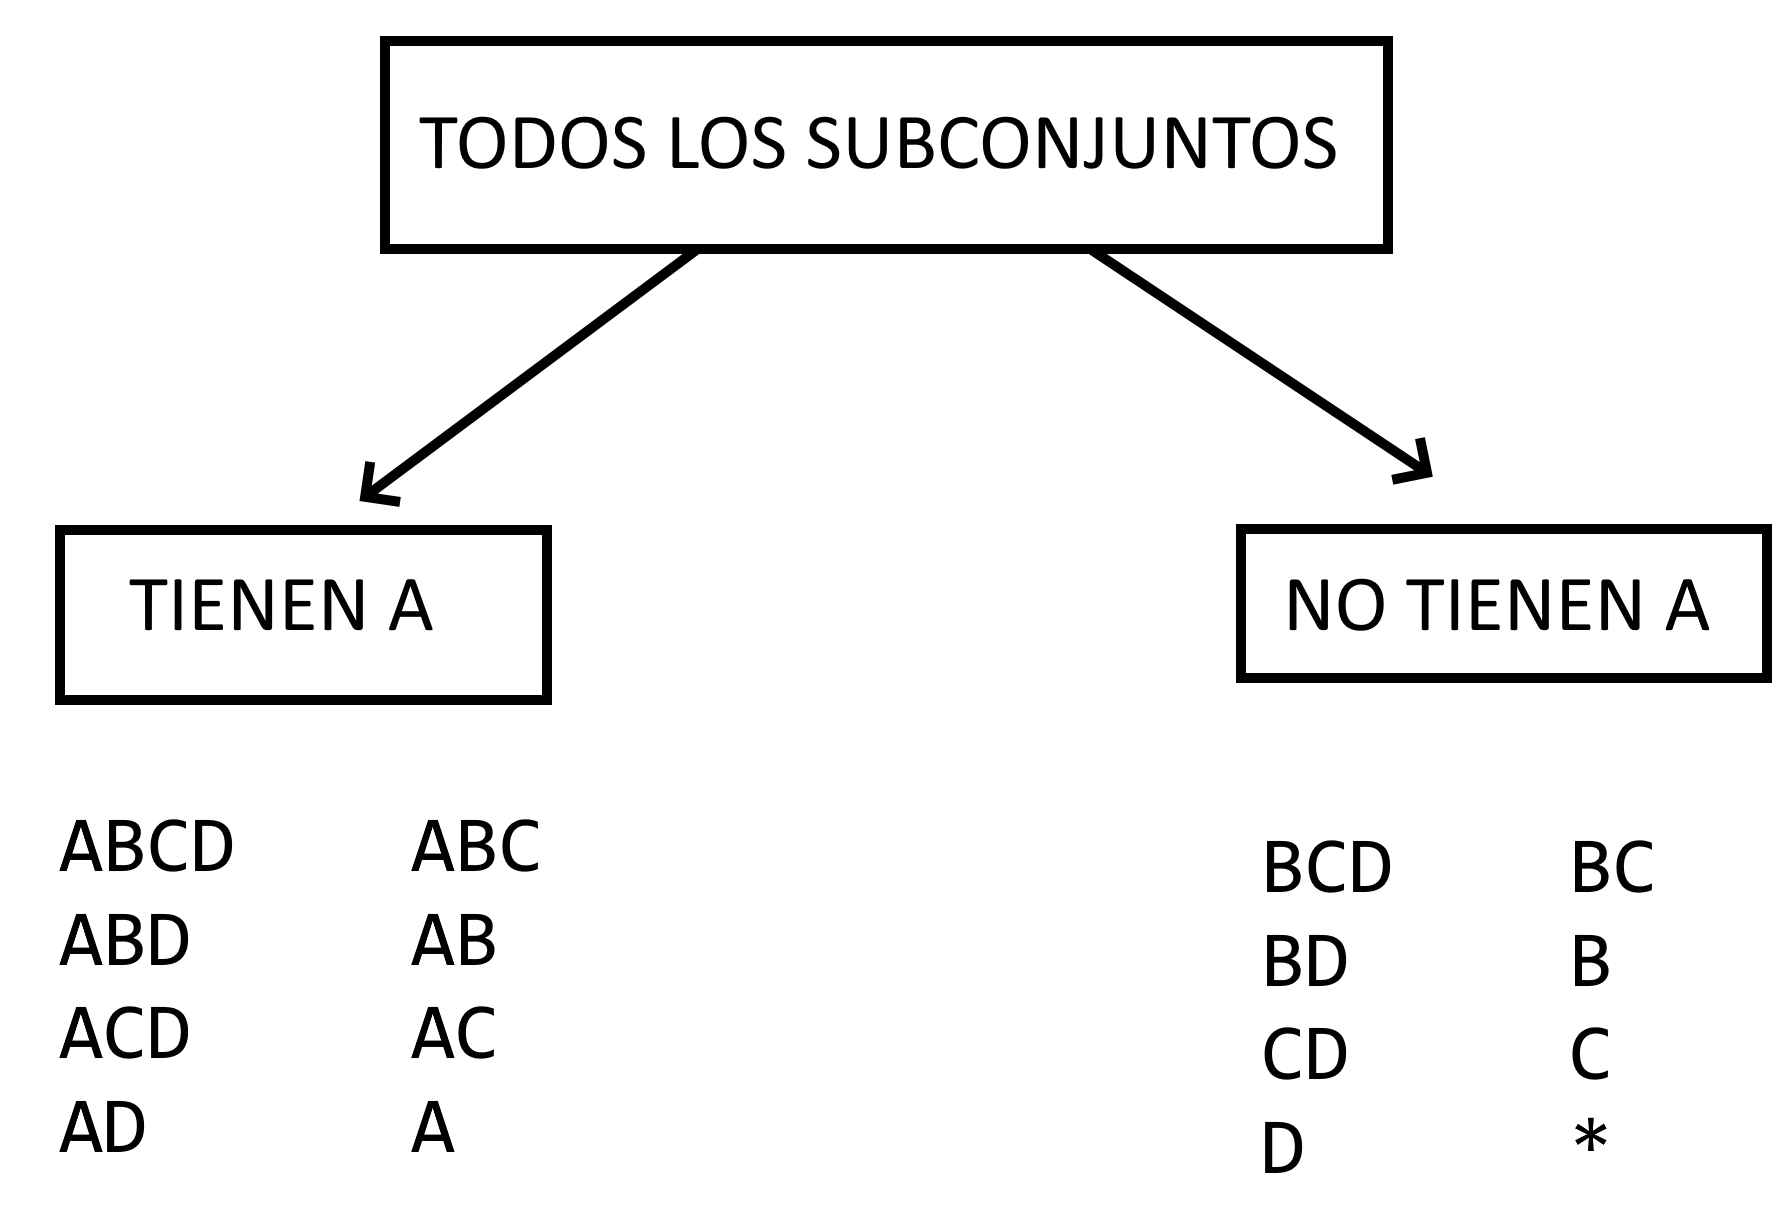
\includegraphics[scale=0.15]{subconjuntos1}
\end{center}

Ahora veamos que para los dos grupos, tenemos todos los 8 subconjuntos para \(BCD\), y lo único que los diferencia es si tienen \(A\) al inicio o no. Si supiéramos cuales son esos subconjuntos para las ultimas 3 letras, podríamos perfectamente construir \(S(ABCD)\), 

En concreto, podemos ver que \(S(ABCD) \) es igual a \(S(BCD)\) con \(A\) al inicio y \(S(BCD)\) sin nada extra. 

Si lo quieres ver en formula sería similar a \(S(ABCD)=A\rightarrow S(BCD) \cup S(BCD)\), donde \(A\rightarrow S(BCD)\) significa agregar \(A\) a todos los subconjuntos en \(S(BCD)\).

Y podemos hacer lo mismo, ver que \(S(BCD)\) es otra vez: los subconjuntos de \(CD\) con B y sin B.

Y de aquí obtenemos nuestro comportamiento recursivo.

Ahora que vemos la recursión, veamos una forma de implementar todo esto para resolver el problema.

Crearemos un metodo construyeSubconjuntos(int pos, int previo) que constuya los subconjuntos usando las letras desde pos hasta \(N-1\).
\pagebreak
\begin{lstlisting}
	#include <iostream>
	using namespace std;
	int N;
	char subconjunto[25];
	
	// pos implica que letra estamos eligiendo si esta o no A=0, B=1, C=2, ...
	// para N=6, pos = 2, es equivalente a  S(CDEF)
	// previo indica cuantas letras se han agregaron a la construccion.
	void construyeSubconjuntos(int pos, int previo) {
		if (pos == N) {
			//Ya no hay mas letras que decidir
			//imprime el subconjunto construido.
			if (previo==0) {
				cout <<"*\n";
			} else {
				cout << subconjunto<<"\n"; 
			}
			return;
		}
		//agrega la letra pos a la construccion
		subconjunto[previo]=pos+'A'; 
		construyeSubconjuntos(pos+1, previo+1); 
		
		// Quita la letra pos de la construccion
		subconjunto[previo]='\0'; 
		construyeSubconjuntos(pos+1, previo); 
		
	}
	
	int main () {
		cin >> N;
		construyeSubconjuntos(0,0);
		return 0;
	}
\end{lstlisting}


De forma que el árbol de la recursión para construyeSubconjuntos(0,0) con \(N=2\) se ve:

\begin{center}
	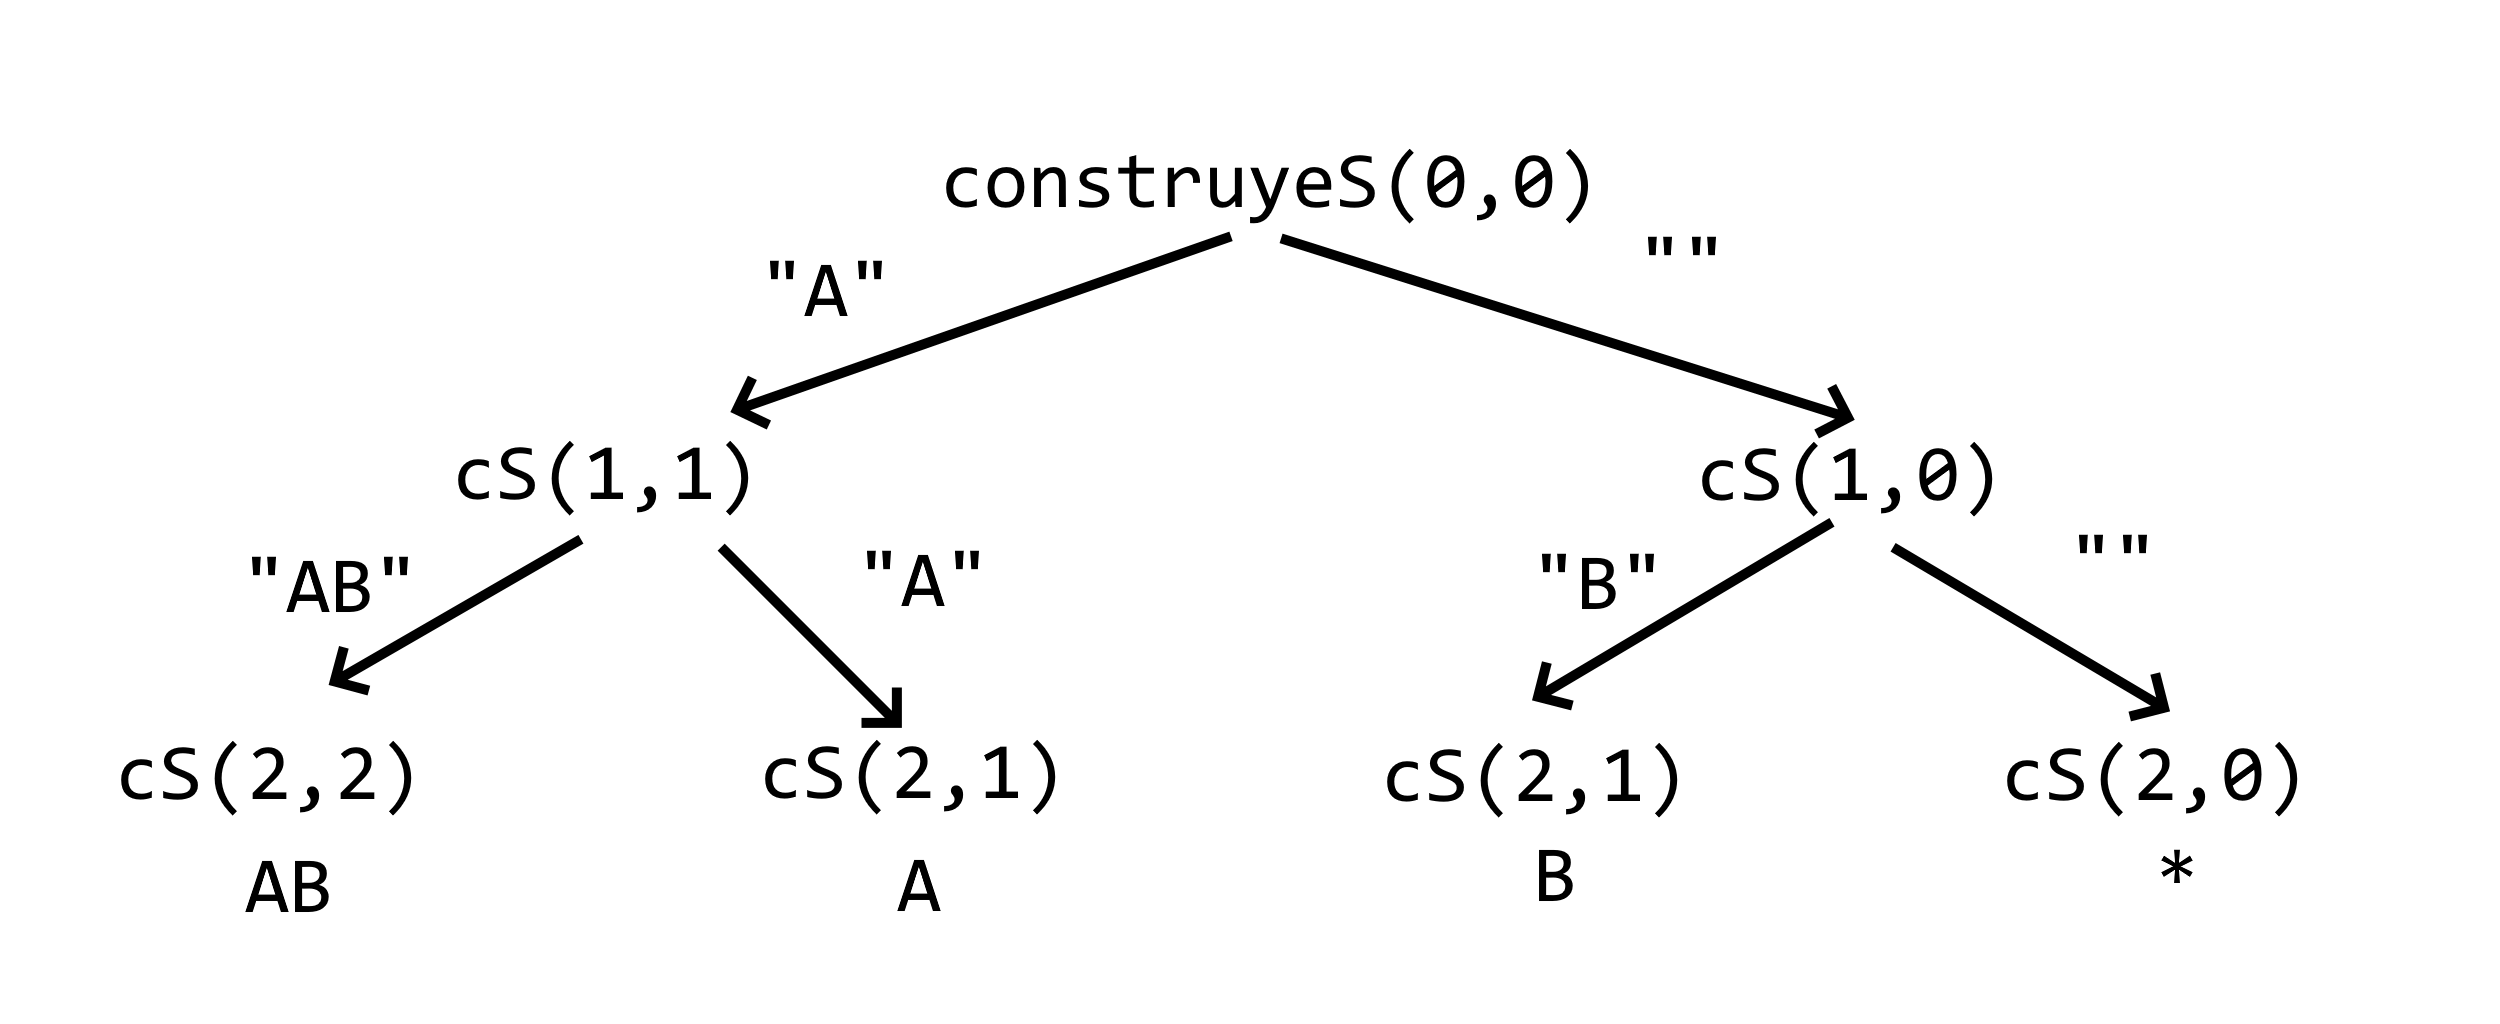
\includegraphics[scale=0.15]{AB}
\end{center} 

\subsection{Complejidad}

a complejidad de este código es igual a la cantidad de subconjuntos que se tienen con \(N\) elementos.

La primera forma de hacerlo es darnos cuenta que cada elemento tiene dos opciones, estar o no estar, por principio multiplicativo vemos que se multiplica por dos tantas veces como elementos tengamos. En total es \(2^N\) 

Esto es observable si recordamos el diagrama de las llamadas recursivas.

Vemos que por cada elemento, se divide en dos, duplicando la cantidad de llamadas en el proceso. En el primer nivel con pos=0, tenemos solo una llamada, con pos=1 tenemos dos, pos=3 obtenemos cuatro y así sucesivamente.

Por lo tanto, la complejidad es \(O(2^N)\), exponencial.

Una vez comprendido esto, pasemos a utilizar esto para resolver problemas.

\subsection{Ejemplo Subconjunto de Suma K}
Fernando ha llegado a la ferretería con su objetivo frecuente de comprar \(K\) tornillos.  Sin embargo, la ferretería no siempre vende cajas con exactamente \(K\) tornillos dentro.

La ferretería tiene \(N\) cajas diferentes en venta, cada uno con \(C_i\) tornillos dentro.

Fernando quiere comprar unas cuantas cajas y obtener \textbf{exactamente} \(K\) tornillos. Por fortuna, esta vez trajo una bolsa y podrá comprar cuantas cajas le sea necesario.

Conociendo las cajas que venden en la Ferretería, determina si Fernando puede comprar los \(K\).

\subsection*{Entrada}
Dos enteros \(N\) y \(K\), la cantidad de cajas en la Ferretería y cuantos tornillos quiere Fernando.

En la siguiente línea vendrán la cantidad de tornillos en cada caja, los valores \(C_i\), separados por espacios.

\subsection*{Salida}
Debes imprimir "SI" en caso de que Fernando pueda comprar exactamente \(K\) tornillos. Caso contrario, imprime "NO".

\subsection*{Ejemplos}
\begin{casebox3}
	\ecase{
		5 10\\
		2 4 5 3 9	
	}
	{SI}
	{
		Compra la primera, tercera\\
		y cuarta caja.
	}
	\ecase{
		5 12\\
		4 5 2 11 3	
	}
	{NO}
	{}
\end{casebox3}
\subsection*{Límites}
\begin{plimits}
	\item \(1\leq N\leq 20 \)
	\item \(1\leq C_i\leq 10^9 \)
	\item \(1\leq K\leq 10^9 \)
\end{plimits}

\subsection*{Solución}
Como siempre, resumamos el problema en menos palabras. En corto, nos preguntan si existe un subconjunto de cajas tal que la suma de sus valores sea exactamente \(K\).

Y como es propio de todos los subtemas de búsqueda completa, veamos todas las posibles soluciones, es decir todos los subconjuntos, hasta que encontremos el que cumpla la condición o nos quedemos sin opciones.

Como ya vimos la forma de iterar por todos los subconjuntos en el ejemplo 3.1, utilicemos esas ideas para resolver este problema.

Lo que podemos hacer es ir construyendo todos los subconjuntos, esta vez en vez de representarlos como una cadena, lo representaremos como su suma. Esto en código se ve:
\newpage
\begin{lstlisting}
	#include<iostream>
	#include<stdlib.h>
	using namespace std;
	int Cajas[25];
	int N;
	long long K;
	// Aqui, llevamos la suma del subconjunto construido
	void buscaSubconjunto(int pos, long long suma) {
		if (pos==N) {
			if (suma == K) {
				/* Encontramos un subconjunto con suma K.
				Imprimmos SI y terminemos el programa */
				cout << "SI";
				exit(0);
			}
			return;
		}
		buscaSubconjunto(pos+1, suma+Cajas[pos]);//Incluyamos pos en el subconjunto
		buscaSubconjunto(pos+1, suma);//Excluyamos pos del subconjunto	
	}
	
	int main () {
		ios_base::sync_with_stdio(0); cin.tie(0);
		cin >> N >>K;
		for (int i=0; i < N; i++) {
			cin >> Cajas[i];
		}
		buscaSubconjunto(0,0);
		//Si llegamos aqui es porque nunca encontramos la respuesta.
		cout << "NO";
		return 0;
	}
\end{lstlisting}

\pagebreak

\section*{Problemas de práctica}
\addcontentsline{toc}{section}{Problemas de práctica}

\begin{exercise}
	\problema[warel-roba-diamantes]{Warel roba diamantes}{\omegauplink{warel-roba-diamantes}}
\end{exercise}

\begin{exercise}
\problema[imprime-binarios]{Imprime números binarios}{\omegauplink{Imprime-binario}}
\end{exercise}
\begin{exercise}	
\problema[imprime-binarios]{Imprime números binarios}{\omegauplink{Imprime-binario}}
\end{exercise}
\begin{exercise}
\problema[reverse-matrix]{Invirtiendo una matriz}{\omegauplink{reverse-matrix}}
\end{exercise}
\section{Forma recursiva}
\markright{FORMA RECURSIVA}

Ahora se verá como crear cualquier búsqueda exhaustiva con recursión, lo cual nos va a servir para cualquier fuerza bruta que no hayamos visto en la lista anterior. Es la forma general de cualquier exhaustiva.

Para resolver esto, imaginaremos que lo que queremos buscar es una una secuencia de valores que cumplan algo. 

Si nos fijamos, todos los ejemplos anteriores fueron eso, buscar una secuencia de valores:

Por ejemplo, en la búsqueda lineal buscábamos una secuencia de un solo número, por ejemplo \([4]\) que representa el valor de la raíz cuadrada de \(16\). Mientras que en las parejas de elementos queríamos una secuencia de dos números que representen la pareja, por ejemplo \([1, 6]\), los indices de un arreglo.

En los ordenes, la permutación tal cual es la secuencia, y en los subconjuntos teníamos una cadena de tamaño n con valores de 0 o 1 representando si un elemento esta o no.

Ahora, la pregunta es ¿cómo buscamos las secuencias de números? para una secuencia lo que podemos imaginar es que tomamos la decisión de cuanto vale el primer elemento de la secuencia, luego elegimos cuanto vale el segundo elemento, luego el tercero, etc. Formando una cadena de decisiones hasta que lleguemos al final de la secuencia.

\begin{center}
	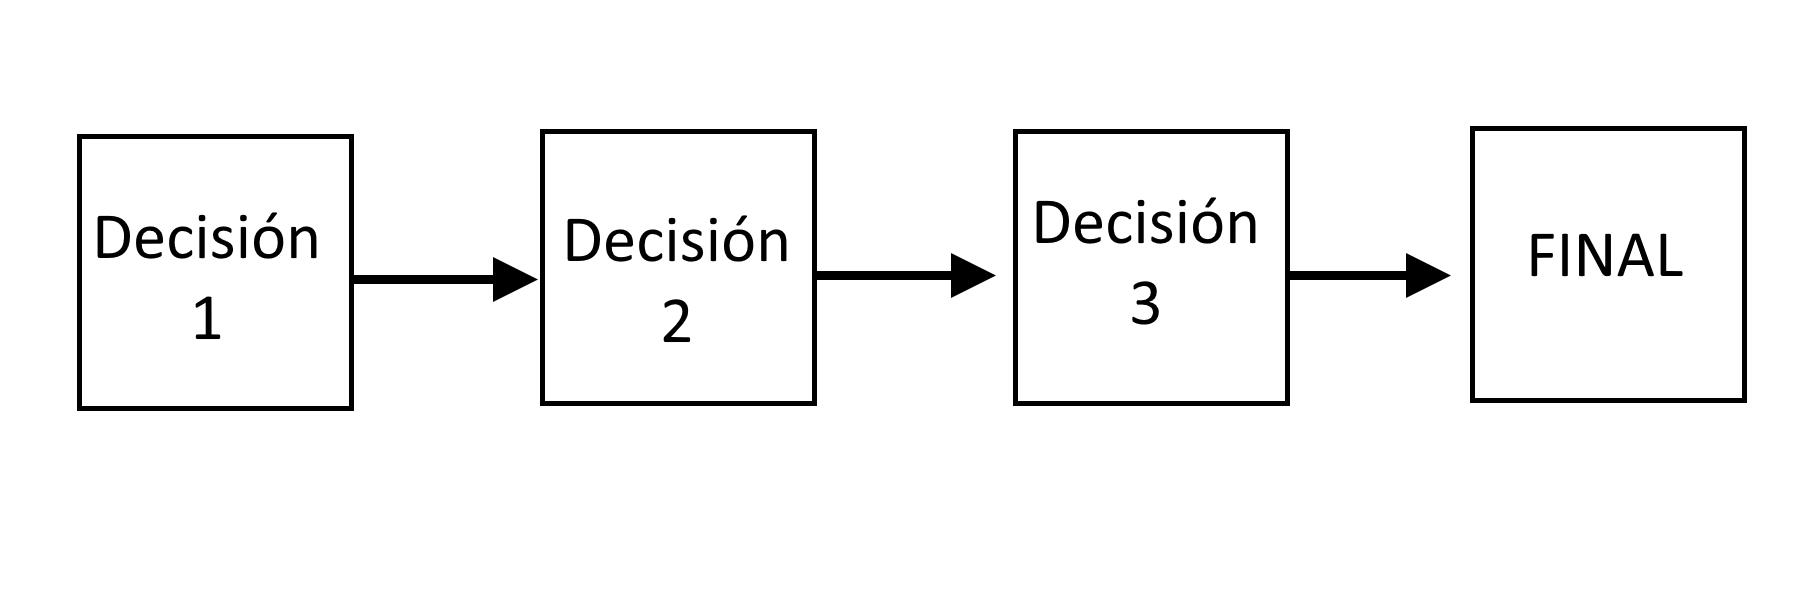
\includegraphics[scale=0.2]{decisiones}
\end{center}

Y la idea de esta búsqueda completa es revisar todas las formas posibles de tomar esta serie de decisiones para encontrar todas las cadenas. 

Para esto hacer esto, cada que tengamos que tomar una decisión, probamos todas las opciones disponibles para ver que producen.

Supongamos que estamos buscando la solución y tenemos una decisión ante nosotros con dos opciones. Lo que la búsqueda exhaustiva hace es ver ``¿qué pasa si elijo la primera opción?" para luego revisar ``¿Y qué sucede con la segunda opción?". Si después hay más decisiones, también explorara todas las opciones que aporten.

De forma que la búsqueda se ve aproximadamente de la siguiente forma:

\begin{lstlisting}
	busqueda(decision, solucion) {
		if (decision es el final) {
			revisar solucion contruida;
			return;
		}		
		//Revisa cada opcion de esta decision:
		for (int i=0; i < decision.opciones; i++) {
			busqueda(siguiente_decision, solucion+ decision.opcion[i] );
		}
	}
\end{lstlisting}

Probablemente reconozcas este código de la forma recursiva de iterar por todos los subconjuntos, esto es porque utilizamos esta técnica para resolver aquella fuerza bruta.

Como es costumbre, veamos ejemplos para entender esto:
\subsection{Ejemplo: Pares de suma K}
Dado un arreglo \(A\) de \(N\) enteros, determina si existe un par \(i\) y \(j\) (\(i<j\)) tal que \(A[i]+A[j]==K\).

\subsection*{Ejemplo}
\begin{casebox2}
	\scase{
		5 8\\
		3 1 2 5 9
	} 
	{SI}
	\scase{
		5 10\\
		3 4 2 12 9
	} {
		NO
	}
	
\end{casebox2}
\subsubsection*{Límites}
\begin{plimits}
	\item \(1\leq N \leq 10^3\)
	\item \(1\leq A[i], K \leq 10^9\)
\end{plimits}

\subsection*{Solución}
Este problema lo vimos en la sección de iterar por pares,lo que debíamos hacer era revisar todas las posibles parejas y ver si existía aquella que sume \(K\).

\begin{lstlisting}
	bool respuesta=false;
	for (int i=0; i < N;i++) {
		for (int j=i+1; j < N; j++) {
			if (A[i]+A[j]==K) {
				respuesta=true;
			}
		}
	}
\end{lstlisting}

Pero ahora pensemos un poco a más profundidad que hace este código.

Primero va revisando todas las opciones de \(i\). Y para cada opción, evalúa todas las opciones para \(j\). 

Tiene que elegir cuanto valen dos valores, probará todos los valores para \(i\) con el primer ciclo, revisando un valor por cada iteración. Y para cada valor de \(i\) probará todos los valores de \(j\) posibles.

Esto se puede ver también con una recursión:
\pagebreak

\begin{lstlisting}
int solucion[3];
bool respuesta=false;
void buscar(int decision) {
	if (decision==3) {
		//Ya tomamos las dos decisiones, cuanto vale i, cuanto vale j. Revisemos esta solucion
		if (A[solucion[1]]+A[solucion[2]]==K) {
			respuesta=true;
		}
		return;
	}
	if (decision == 1) {
		//toca decidir cuanto vale i. Como esto es busqueda completa, revisaremos cada opcion.
		for (int i=0;i < N; i++) {
			solucion[decision]=i;//agregar i a la solucion
			buscar(decision+1);	
			solucion[decision]=-1;//quitar i de la solucion
		}
	} else {
		//toca decidir cuanto valdra j. Probemos todos los valores
		for (int j= solucion[1]+1; j< N;j++) {				
			solucion[decision]=i;//agregar j a la solucion
			buscar(decision+1);
			solucion[decision]=i;//quitar j.
		}
	}
}


int main() {
	[...]
	buscar(1);
	cout << "NO";
	return 0;
}
\end{lstlisting}

Estos dos códigos siguen la misma idea de obtener los pares fijando primero un valor de \(i\), y  luego fijando un valor para \(j\); solo lo realizan de una forma diferente.

\textbf{Consejo:} Entiende porque los dos códigos resuelven el problema con la misma idea antes de continuar, prueba a ejecutar ambos a mano con lápiz y papel.

Básicamente el primer código hace lo siguiente para explorar todos los pares:
\begin{center}
	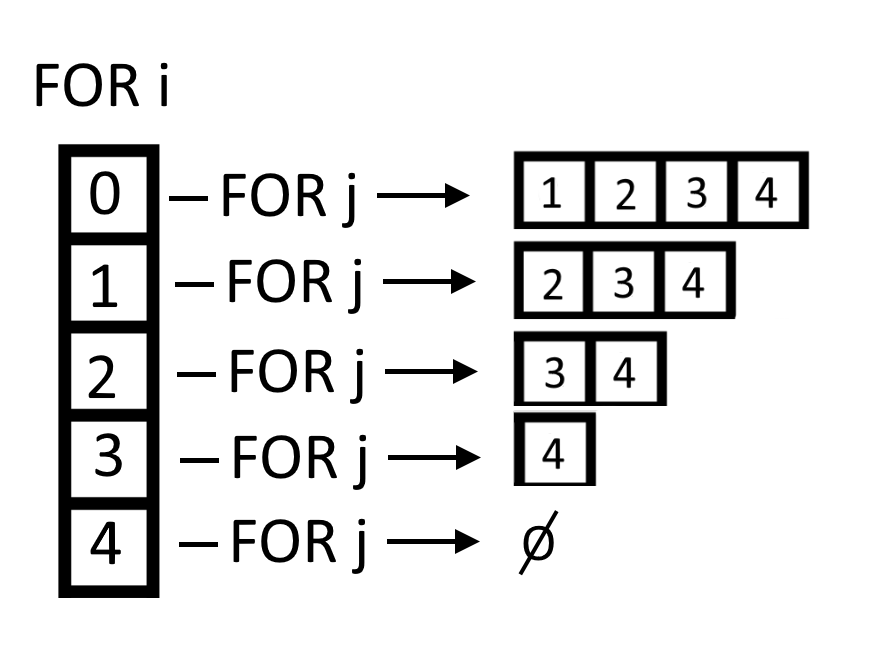
\includegraphics[scale=0.3]{forbrute}
\end{center}

Donde para cada elemento de la lista de valores de \(i\), prueba los valores de \(j\).

Mientras que el segundo hace recursión para obtener todos los pares posibles.

\begin{center}
	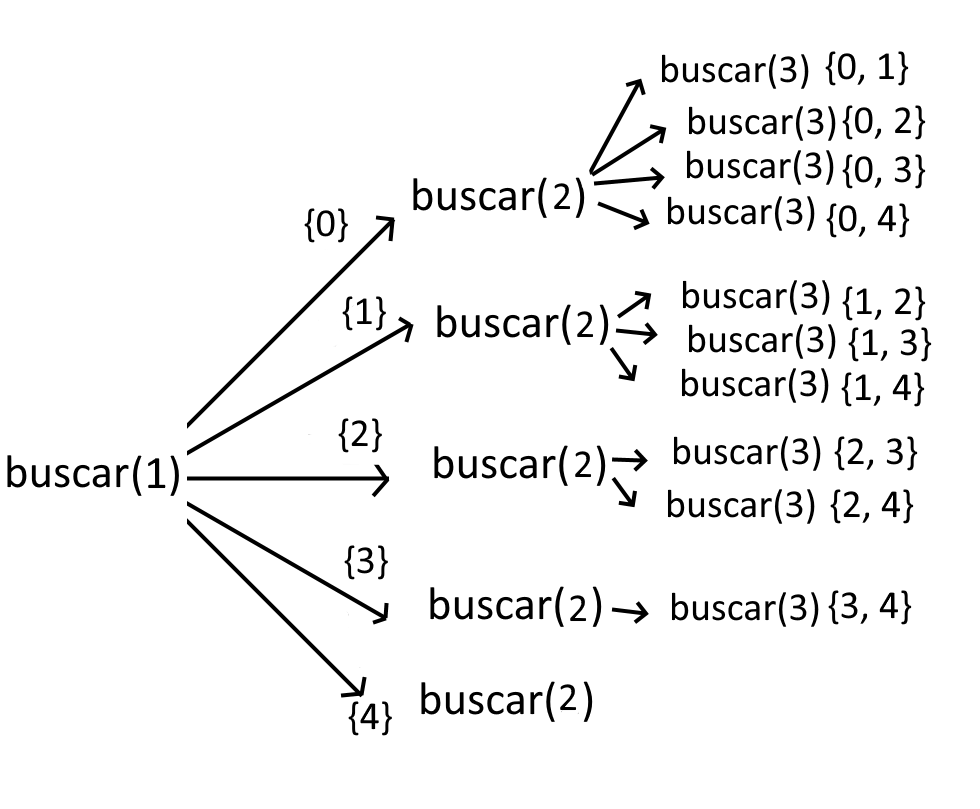
\includegraphics[scale=0.3]{paresrec}
\end{center}

Ambos son búsquedas exhaustivas que exploran todas las formas de tomar las decisiones de elegir \(i\) y luego \(j\).

Veamos otro ejemplo:

\subsection{Ejemplo: Dividir en tres grupos}
Una clase se ha juntado para jugar LaserTag. Por el diseño del lugar donde van a jugar han decidido formar tres equipos, pero quieren que los jugadores sean repartidos justamente.

La clase consiste de \(n\) estudiantes. El estudiante \(i\) tiene \(a_i\) habilidad para el LaserTag. 

Los equipos están repartidos de forma justa si la suma de la habilidad de sus integrantes es igual para los tres equipos y nadie se queda sin equipo.

Determina si se puede formar los equipos de forma justa y si sí, determina la repartición.

\textbf{Entrada}\\
Un entero \(n\), indicando la cantidad de estudiantes en la clase.

La segunda línea tendrá \(n\) enteros \(a_1, a_2, \ldots, a_n\), donde \(a_i\) es la habilidad del estudiante \(i\).

\textbf{Salida}\\
Si no se puede hacer la repartición imprime \verb|NO|.

En caso de que se pueda, en la primera línea imprime \verb|SI|.

En la segunda línea imprime \(n\) enteros. El \(i\)-ésimo entero sera 1, 2 o 3 dependiendo de a que equipo va el estudiante \(i\). 

Si hay varias soluciones, se acepta cualquiera.

\begin{samepage}
	\textbf{Ejemplo}\\
	\begin{casebox3}
		\ecase{
			6\\
			3 1 6 2 4 2  
		}{
			SI\\
			1 1 3 2 2 1
		}{
			El primer equipo tiene una habilidad\\ de
			\(3+1+2\).
			\\
			\\
			El segundo tiene habilidad de \(2+4\).
			\\
			\\
			Y el tercer equipo tiene un\\ integrante de \(6\).
		}
		\ecase{
			6\\
			2 1 5 2 3 4
		}{NO}{No se puede repartir a\\ los estudiantes justamente.}
	\end{casebox3}

\end{samepage}

\textbf{Límites}
\begin{plimits}
	\item \(1\leq N \leq 15\)
	\item \(1\leq a_i \leq 10^6\)
\end{plimits}

ENLACE: TODO

\subsection*{Solución}

Como siempre, antes de leer la solución te invitamos a que trates de resolver el problema por un rato.

Entonces, podemos pensarlo como que tenemos \(N\) decisiones, donde cada decisión es ¿A que equipo envío al estudiante \(i\)?

Y lo podemos imaginar como que los estudiantes se forman delante de nosotros y les vamos diciendo: "Equipo 1, equipo 2, equipo 1, equipo 3, ... ".

Entonces, podemos hacer un código que haga eso, que vaya tomando las decisiones de enviar a cada estudiante al equipo 1, 2 o 3.

Para esto crearemos la función repartir(int c, int equipo1, int equipo2, int equipo3) que se encargara de decidir a cual equipo mandar al estudiante \(c\). 
Y llevaremos cuenta de cuanta habilidad lleva cada equipo hasta ahora.

Además usaremos un arreglo \verb|reparticion[]| para llevar cuenta de a que equipo mandamos cada estudiante.

\pagebreak

\begin{lstlisting}
	int n;
	int a[16];
	int reparticion[16];
	void repartir(int c, int equipo1, int equipo2, int equipo3) 
	{
		//Mandar el estudiante c al equipo1:
		reparticion[c]=1;
		repartir(c+1, equipo1+a[c], equipo2, equipo3);
		
		//Mandar el estudiante c al equipo2:
		reparticion[c]=2;
		repartir(c+1, equipo1, equipo2+a[c], equipo3);
		
		//Mandar el estudiante c al equipo2:
		reparticion[c]=3;
		repartir(c+1, equipo1, equipo2, equipo3+a[c]);
	}
\end{lstlisting}

Ahora, le falta la condición de paro. Esto será en el momento que ya no tengamos estudiantes que repartir, cuando \(c=n\).

Además, aprovecharemos allí para validar que la repartición sea justa. Si lo es, imprimiremos esta construcción como respuesta y terminaremos el programa.
\pagebreak
\begin{lstlisting}
	int n;
	int a[16];
	int reparticion[16];
	void repartir(int c, int equipo1, int equipo2, int equipo3) 
	{
		if (c==n) {
			if (equipo1==equipo2 && equipo1==equipo3) {
				cout << "SI\n";
				for (int i =0;i<n; i++) 
				cout << reparticion[i]<<" ";					
				exit(0);
			}
			return;
		}
		//Mandar el estudiante c al equipo1:
		reparticion[c]=1;
		repartir(c+1, equipo1+a[c], equipo2, equipo3);
		
		//Mandar el estudiante c al equipo2:
		reparticion[c]=2;
		repartir(c+1, equipo1, equipo2+a[c], equipo3);
		
		//Mandar el estudiante c al equipo2:
		reparticion[c]=3;
		repartir(c+1, equipo1, equipo2, equipo3+a[c]);
	}
	int main() {
		ios_base::sync_with_stdio(0); cin.tie(0);
		cin >> n;
		for (int i =0; i< n; i++) {
			cin >> a[i];
		}
		repartir(0, 0, 0, 0);
		cout << "NO";
	}
	
\end{lstlisting}

\subsection{Complejidad}

La complejidad de una búsqueda exhaustiva varia mucho dependiendo de que tipo de solución se esta buscando, en el primer ejemplo terminamos con una complejidad de \(O(N^2)\). 

Pero la complejidad del ejemplo anterior es \(O(3^N)\). Esto es porque la complejidad de la búsqueda exhaustiva es \(O(candidatos)\) y en este caso, las formas de repartir se multiplican por tres por cada estudiante que se agregue a la clase, ya que tenemos todas las opciones de equipos anteriores, pero unas con el nuevo en el 1, otros con el equipo 2, y otra vez con el estudiante en el 3.


\section*{Problemas de práctica}
\addcontentsline{toc}{section}{Problemas de práctica}
\begin{exercise}
	\problema{Encontrar posición en un arreglo}{TODO}

	NOTA: Utiliza recursión.
\end{exercise}

\begin{exercise}
	\problema{Contando LaserTag justos}{TODO}
\end{exercise}
\begin{exercise}
	\problema[torre-I]{Subiendo la torre}{TODO}
\end{exercise}

\begin{exercise}
	\problema{Mapas}{\omegauplink{OMI-2020-Mapas}}
\end{exercise}



\section*{Problemas de práctica}
\addcontentsline{toc}{section}{Problemas de práctica}
\markright{Problemas de práctica}

\begin{exercise}
	\problema{Contando LaserTag justos}{TODO}
\end{exercise}

\begin{exercise}
	\problema[torre-I]{Subiendo la torre}{TODO}
\end{exercise}

\begin{exercise}
	\problema{Mapas}{\omegauplink{OMI-2020-Mapas}}
\end{exercise}

\begin{exercise}
	\problema[problemas/frecuencia-de-k]{TODO Frecuencia de K}{\omegauplink{frecuencia-de-k}}
\end{exercise}

\begin{exercise}
	\problema[problemas/multiplos-de-cinco]{TODO Multiplos de cinco}{\omegauplink{multiplos-cinco}}
\end{exercise}

\begin{exercise}
	\problema[problemas/divisores]{TODO: Divisores del entero}{\omegauplink{divisores-entero}}
\end{exercise}

\begin{exercise}
	\problema[problemas/suma-de-digitos]{A la suma de digitos}{\omegauplink{m-suma-digitos}}
\end{exercise}

\begin{exercise}
	\problema[problemas/escalera-de-fer]{Escalera de fer}{TODO}
\end{exercise}

\begin{exercise}
	\problema[problemas/bicicleta-de-karel]{Bicicleta de Karel I}{\omegauplink{bicicleta-de-karel-i}}
\end{exercise}

\begin{exercise}
	\problema[problemas/contar-capicuas]{Contar capicúas}{\omegauplink{Contar-capicuas}}
\end{exercise}

\begin{exercise}
	\problema[problemas/cuenta-primos]{Cuenta primos}{\omegauplink{Cuenta-primos}}
\end{exercise}

\begin{exercise}
	\problema[inversiones-arreglo]{TODO Inversiones en el arreglo}{\omegauplink{inversiones-arreglo}}
\end{exercise}

\begin{exercise}
	\problema[contar-sumas-pares]{TODO Puntuación de la ferretería}{\omegauplink{contar-sumas-pares}}
\end{exercise}

\begin{exercise}
	\problema[algofashion-fibo]{TODO Números de moda}{\omegauplink{moda-fibonacci}}
\end{exercise}

\begin{exercise}
	\problema[terreno-valioso]{TODO Terreno más valios}{\omegauplink{TODO terreno-valioso}}
\end{exercise}

\begin{exercise}
	\problema[suma-modulo-k]{TODO Suma modular}{\omegauplink{TODO suma-modulo-k}}
\end{exercise}

\begin{exercise}
	\problema[warel-roba-diamantes]{Warel roba diamantes}{\omegauplink{warel-roba-diamantes}}
\end{exercise}

\begin{exercise}
	\problema[imprime-binarios]{Imprime números binarios}{\omegauplink{Imprime-binario}}
\end{exercise}

\begin{exercise}
	\problema[reverse-matrix]{Invirtiendo una matriz}{\omegauplink{TODO reverse-matrix}}
\end{exercise}



\chapter[Búsqueda con podas]{Búsqueda con podas\\ Backtracking}

Sigamos con otra búsqueda que evita probar absolutamente todo el espacio de búsqueda, en este caso es la búsqueda de vuelta a atrás, o backtracking en inglés.

Esta búsqueda es similar a la búsqueda exhaustiva, pero estando atentos a no explorar candidatos en los que nos demos cuenta que no encontraremos lo que buscamos.

Como acostumbramos veamos un ejemplo.

\section*{Ejemplo: Subconjunto de suma K}

Dada una lista de \(N\) enteros positivos, determina si existe un subconjunto que sus elementos sumen \(K\).

\textbf{Entrada}\\
Dos enteros \(N\) y \(K\) --- La cantidad de enteros y la suma que queremos.

En la segunda línea hay \(N\) enteros \(A_1, A_2, \ldots A_N\) --- Los valores de la lista.
\textbf{Salida}\\
Imprime \verb|SI| en caso de que exista un subconjunto de suma \(K\), o imprime \verb|NO| en caso contrario.

\textbf{Ejemplos}\\
\begin{casebox3}
	\ecase{
	4 12\\
	5 8 3 1 7	
	} {
	SI
	}
	{
		\(5+7=12\)
	}
	\ecase{
		6 11\\
		10 5 2 3 5 7
	} {
		NO
	}
	{
	}
	\ecase{
	4 22\\
	5 5 5 11 
	} {
	NO
	}
	{	
	}
\end{casebox3}

\textbf{Límites}
\begin{plimits}
	\item \(1\leq N,K \leq 200\)
	\item \(1\leq A_i \leq 200\)
\end{plimits}
	
\textbf{Subtareas}
\begin{plimits}
	\item (30 pts) \(1\leq N \leq 20\)
	\item (30 pts)
	\begin{plimits}
		\item \(1\leq N \leq 30\)
		\item \(1\leq K \leq 9\)		
	\end{plimits}
	\item (40 pts) Sin restricciones adicionales
\end{plimits}

\subsection*{Solución}
Vamos a ir construyendo una solución desde la fuerza bruta hasta obtener la de 100 puntos.

\subsubsection*{Fuerza bruta}
La fuerza bruta es crear todos los subconjuntos posibles, viendo si la suma es lo que queremos o no, recordemos que en código se ve:

\begin{minipage}{\linewidth}
\begin{lstlisting}
void buscar(int posicion, int suma) {
	if (posicion==N) {
		if (suma==K) {
			cout << "SI";
			exit(0);
		}
		return;
	}
	//prueba a incluir arr[pos]
	buscar(posicion+1, suma+arr[posicion]);
	
	//prueba a excluir arr[pos]
	buscar(posicion+1, suma);
}
\end{lstlisting}
\end{minipage}

Esta búsqueda nos produce el siguiente diagrama de recursión en el caso ejemplo uno. Cada llamada recursiva es representada por dos números, el primero es posición y el segundo es suma.


\Tree [.buscar(0,0) 
	[.1\\5 
		[.2\\13 
			[.3\\16
				[.4\\17 
					5\\24 
					5\\17
				]
				[.4\\16
					5\\23
					5\\16
				]
			]
			[.3\\13
				[.4\\14
					5\\21
					5\\14
				]
				[.4\\13
					5\\20
					5\\13
				]
			]
		]
		[.2\\5
			[.3\\8
				[.4\\9
					5\\16
					5\\9				
				]
				[.4\\8
				5\\15
				5\\8				
				]
			]			
			[.3\\5
				[.4\\6
					5\\13
					5\\6
				]
				[.4\\5
					\textbf{5}\\\textbf{12}
				]
			]		
		]
	]	
]




En total, se requirió de 31 llamadas recursivas y revisamos 15 subconjuntos, ¿pero realmente fue necesario hacer todo lo que hicimos?

\subsection*{Primera poda}
Pongamos atención en la llamada de \lstinline|buscar(2, 13)|, desde aquí hacemos 14 llamadas recursivas, que si lo pensamos ya son innecesarias. Si la suma ya supero 12, que es lo que buscamos y no hay números negativos, entonces no importa que hagamos, jamas encontraremos 12.

Por lo tanto, la primera forma de mejorar la fuerza bruta es detener la búsqueda si superamos \(K\). Esto se ve en código:

\begin{minipage}{\linewidth}
	\begin{lstlisting}
		void buscar(int posicion, int suma) {
			if (suma > K) {
				return;
			}
			if (posicion==N) {
				if (suma==K) {
					cout << "SI";
					exit(0);
				}
				return;
			}
			//prueba a incluir arr[pos]
			buscar(posicion+1, suma+arr[posicion]);
			
			//prueba a excluir arr[pos]
			buscar(posicion+1, suma);
		}
	\end{lstlisting}
\end{minipage}

De forma que ahora el diagrama de la recursión es mucho menor.

\Tree [.buscar(0,0) 
[.1\\5 
		[.2\\13 		
		]
		[.2\\5
			[.3\\8
				[.4\\9
					5\\16
					5\\9				
				]
				[.4\\8
					5\\15
					5\\8				
				]
			]
			[.3\\5
				[.4\\6
					5\\13
					5\\6
				]
				[.4\\5
					\textbf{5}\\\textbf{12}
				]
			]			
		]
	]	
]

Esta poda nos permite sacar la segunda subtarea, esto es porque como \(K\) vale a lo más \(9\), la cantidad de subconjuntos por explorar son aquellos con \(9\) elementos o menos, los cuales para \(n=30\) hay \(22,964,087\), esto lo podemos comprobar con una búsqueda que cuente la cantidad de subconjuntos de menos de \(9\) elementos, o con fórmulas matemáticas que veremos más adelante.

A esta forma de evitar visitar candidatos le llamamos poda, porque estamos podando ramas del diagrama y reduciendo el volumen de búsqueda. Igual que podar un árbol reduce la cantidad de hojas y el volumen de un árbol.

\subsection*{Segunda poda}
Esta no es la única forma de podar, también podemos cortar la búsqueda en con información de lo que ya hemos explorado.

Para ver esto, veamos el tercer caso ejemplo.


\Tree[.0\\0
	[.1\\5
		[.2\\10
			[.3\\15
				4\\26
				4\\15
			]
			[.3\\10
				4\\21
				4\\10			
			]
		]	
		[.\textbf{2}\\\textbf{5}
			[.\textbf{3}\\\textbf{10}
				\textbf{4}\\\textbf{21}
				\textbf{4}\\\textbf{10}			
			]
			[.\textbf{3}\\\textbf{5}
				\textbf{4}\\\textbf{16}
				\textbf{4}\\\textbf{5}
			]				
		]
	]
	[.1\\0
		[.\textbf{2}\\\textbf{5}
			[.\textbf{3}\\\textbf{10}
				\textbf{4}\\\textbf{21}
				\textbf{4}\\\textbf{10}
			]
			[.\textbf{3}\\\textbf{5}
				\textbf{4}\\\textbf{16}
				\textbf{4}\\\textbf{5}
			]
		]
		[.2\\0
			[.3\\5
				4\\16
				4\\5
			]
			[.3\\0
				4\\11
				4\\0
			]
		]
	]	
]

Este diagrama no es afectado por la poda anterior, pero vamos a introducir una nueva poda. Para esto, probablemente te fijaste en que en el diagrama anterior, resaltamos dos ramas del diagrama en negritas.

El motivo por el cual están calcadas es porque son iguales, inician con buscar(2, 5) para llamar a buscar(3, 10) y buscar(3, 5), etc. Y como son iguales, entonces la segunda vez que lo exploremos, ¿podremos ahora encontrar la respuesta? Claro que no, vamos a ver lo que ya habíamos revisado antes.

Por esto, la segunda poda será que en caso de llegar a un buscar con un valor repetido de posicion  y suma, detener la búsqueda.

En código se ve:

\begin{minipage}{\linewidth}
	\begin{lstlisting}
bool marcas[250][250];
void buscar(int posicion, int suma) {
	if (suma > K) 
		return;	
	if (marcas[posicion][suma]) 
		return;
	marcas[posicion][suma]=true;//Marcamos esta pareja de (pos, suma) como ya explorado para no repetir.
	if (posicion==N) {
		if (suma==K) {
			cout << "SI";
			exit(0);
		}
		return;
	}
	//prueba a incluir arr[pos]
	buscar(posicion+1, suma+arr[posicion]);
	
	//prueba a excluir arr[pos]
	buscar(posicion+1, suma);
}
	\end{lstlisting}
\end{minipage}

Y esto produce el siguiente diagrama, donde marcamos con negritas las ramas podadas:

\Tree[.0\\0
[.1\\5
[.2\\10
[.3\\15
4\\26
4\\15
]
[.3\\10
4\\21
4\\10			
]
]	
[.2\\5
[.\textbf{3}\\\textbf{10}		
]
[.3\\5
4\\16
4\\5
]				
]
]
[.1\\0
[.\textbf{2}\\\textbf{5}
]
[.2\\0
[.\textbf{3}\\\textbf{5}
]
[.3\\0
4\\11
4\\0
]
]
]	
]

Esta poda nos pasa de 31 llamadas recursivas y 16 subconjuntos revisados, a solo usar 21 llamadas y revisar 7 subconjuntos.

Esta poda en concreto nos reduce la complejidad a \(O(NK)\), esto es porque vamos a explorar solo cuando los argumentos aparecen por primera vez. Los valores de posición son de \(0\) a \(N\) y los la suma tiene rango de \(0\) a \(K\). Lo cual implica que en total tenemos \((N+1)(K+1)\) posibles pares de valores. 

Hay llamadas repetidas para los pares, pero estas no hacen nada ya que son podadas de forma inmediata, además, estas solo pueden ser llamadas por un buscar no podado.

Complejidad de \(O(NK)\) corre en tiempo sin problemas para los 100 puntos.

Veamos otro ejemplo.

\section*{Ejemplo: Explorando una matriz}

Un explorador tiene que decidir donde construir un camino para llegar de un punto \(A\) a un punto \(B\). 

Para auxiliarse el explorador ha hecho un mapa con los obstáculos que existen. Cuadriculó su mapa y quiere un camino que pase por el menor número de cuadros. El camino sólo puede ir de un cuadro a otro si tienen un lado en común, es decir, no puede avanzar en diagonal, y no puede pasar por un cuadro que contenga un obstáculo. 

Cada cuadro del mapa se identifica por sus coordenadas, primero la fila y después la columna. Las filas están numerados de arriba hacia abajo iniciando con el \(0\). Las columnas están numeradas de izquierda a derecha iniciando con el \(0\).

Escribe un programa que dado un mapa con obstáculos encuentre el menor número de cuadros por los que debe pasar un camino que vaya del punto \(A\) al punto \(B\), incluyendo a los cuadros que contienen a \(A\) y a \(B\).

\textbf{Entrada}\\
En la primera línea los enteros \(N\) y \(M\) el número de filas y columnas del mapa. En cada una de las siguientes.

En las siguientes \(N\) líneas hay \(M\) enteros que pueden ser \verb|0| ó \verb|1|. Es \verb|0| si no hay obstáculo en el cuadro correspondiente y \verb|1| si lo hay.

En la siguiente línea (la penúltima) la fila y columna del punto \(A\).

En la última línea la fila y columna del punto \(B\).

\textbf{Salida}\\
En la primera linea el número de cuadros por los que pasa un camino mínimo entre \(A\) y \(B\)

\textbf{Ejemplo}\\
\begin{casebox2}
	\scase{
	4 5\\
	0 1 0 0 0\\
	0 0 1 1 0\\
	0 1 0 0 0\\
	0 0 0 0 0\\
	3 1\\
	0 2	
	}{9}
\end{casebox2}

\textbf{Límites}
\begin{plimits}
	\item \(1 \leq N, M\leq 50\)
\end{plimits}

Fuente: OMI 1996, Modificado subtask A

\omegauplink{OIEG2013SSC}

\subsection*{Solución}
Comencemos con la fuerza bruta, básicamente, buscaremos la secuencia de pasos más corta para llegar desde el punto \(A\) hasta el punto \(B\).

Para esto, una observación clave es que ningún camino que sea el más corto pasa dos veces por la misma casilla, esto es porque es innecesario caminar en círculos.

Esto implica que la distancia a lo más usa todas las casillas, esto es \(50\times50=2500\).

Ahora, la fuerza bruta la haremos con una función recursiva que vaya probando todas las secuencias de movimientos posibles, llevando cuenta de las coordenadas de donde va y cuantos pasos ha dado:

\begin{minipage}{\linewidth}
\begin{lstlisting}
int N, M;
int respuesta=1e9;
int destino_i, destino_j;
int marcas[55][55];
void explorar(int pos_i, int pos_j, int pasos) {
	if (pos_i < 0 || pos_i >=N)
		return;//Estas fuera del mapa
	if (pos_j < 0 || pos_j >=M)
		return;//Estas fuera del mapa
	if (pos_i==destino_i && pos_j == destino_j) {
		//Comparar respuesta con la que encontramos
		if (respuesta > pasos)
			respuesta=pasos;
		return;
	}
	if (mapa[pos_i][pos_j])return;
	if (marcas[pos_i][pos_j]) return;
	marcas[pos_i][pos_j]=true; //Marcar para no pasar por aqui otra vez.	
	explorar(pos_i-1, pos_j, pasos+1);//arriba
	explorar(pos_i+1, pos_j, pasos+1);//abajo
	explorar(pos_i, pos_j-1, pasos+1);//izquierda
	explorar(pos_i, pos_j+1, pasos+1);//derecha	
	marcas[pos_i][pos_j]=false; //Desmarcar para permitir pasar por aqui en otros caminos.	
}
int main() {
	cin >> N >>M;
	[...]
	int pi, pj;
	cin >> pi >> pj;
	cin >> destino_i>>destino_j;
	explorar(pi, pj, 1);
	cout << respuesta;
}

\end{lstlisting}
\end{minipage}

Esta fuerza bruta prueba todos los caminos posibles del punto \(A\) al punto \(B\), pero es excesivamente lenta y obtenemos 0 puntos, necesitamos mejorarla.

La primera poda que podemos hacer es que si en algun momento llevamos más pasos que la respuesta encontrada hasta ahora, nos detengamos.

\begin{lstlisting}
	if (pasos >=respuesta) return;
\end{lstlisting}

Con esta idea mejoramos a 25 puntos, pero todavía podemos mejorar.

Para esto, veamos que si en algun momento llegamos a la casilla \((i, j)\) con 20 pasos y luego llegamos con 50, de aquí no podremos encontrar un camino más rápido al punto \(B\), pues todos los caminos desde aquí ya fueron explorados y de forma mejor.

Entonces, añadiremos para cada casilla un marcador de con que tiempo llegamos y solo exploraremos una casilla si llegamos a ella más rápido que antes.
\begin{lstlisting}
if (tiempo[pos_i][pos_j]<=pasos) return;
tiempo[pos_i][pos_j]=pasos;
\end{lstlisting}

Esta segunda poda nos pasa la complejidad a: \(O(distanciaMaxima\times N \times M)\) y como ya vimos, distanciaMaxima es \(N\times M\), por lo tanto la complejidad es \(O((NM)^2)\), lo cual equivale a \(50^4=6,250,000\) que corre en tiempo.

Esta complejidad es resultado de que cada casilla es explorada a lo más la distancia máxima de veces.
\pagebreak
\section{Código general}

Entonces, un código de backtracking se va a ver con la siguiente forma:
\begin{lstlisting}
void buscar(solucion) {
	if (se poda solucion)
		return;
	if (solucion es valida) {
		registrar solucion;
	}
	buscar(soluciones siguientes)
}
\end{lstlisting}

\section*{Problemas de práctica}

\begin{exercise}
	\problema{Suma de digitos}{\omegauplink{Suma-de-digitos}}	
\end{exercise}

\begin{exercise}
	\problema{8 Reinas}{\omegauplink{8Reinas}}
\end{exercise}

\chapter{Exploración}

Para los problemas de grafos ser capaz de recorrer los vértices del grafo en búsqueda de información nos ofrece muchas herramientas para estos problemas.  

Para esto recordemos las búsquedas que vimos en el capítulo 2, la búsqueda exhaustiva, DFS y BFS; ya que los recorridos básicos de un grafo son estos mismos.

El primer recorrido que veremos es la DFS, recordemos un poco acerca de como se comporta.

\chapter{DFS}

La DFS o búsqueda en profundidad es una técnica que explora un grafo vértice por vértice. Útil para encontrar vértices alcanzables y hacer coloreo. 

Iniciando en un primer nodo, en cada paso busca un vecino del nodo actual y lo explora, si no encuentra un vértice sin explorar, regresa por el camino que tomo en búsqueda de vértices que se haya dejado.


\begin{center}
	DIBUJO TODO
\end{center}


\pagebreak

Y el código de una DFS es igual al que ya habíamos visto previamente.

\begin{lstlisting}
	vector<int> adyacencia[100050];
	bool visitado[100050];
	void DFS(int vertice) {
		visitado[vertice]=true;
		for (int i=0; i < adyacencia[vertice].size(); i++) {
			int vecino = adyacencia[vertice][i];
			if (!visitado[vecino]) {
				DFS(vecino);
			}
		}
	}
\end{lstlisting}

\section*{Ejemplo: Conectividad}

Pedro vive en un pequeño país de Oceanía, formado por \(N\) islas enumeradas del \(1\) al \(N\). Entre estas islas hay \(M\) túneles submarinos que las conectan, permitiendo manejar un coche de isla a isla. 

Pedro quiere saber si puede tomar su coche de la isla \(a\) a la isla \(b\).

\textbf{Entrada}\\
En la primera línea tendrás cuatro enteros \(N\), \(M\), \(a\) y \(b\) --- El número de islas en el país, el número de túneles, la isla donde Pedro está y la isla a donde quiere ir.

En cada una de las siguientes \(M\) líneas vendrá la descripción de un túnel, cada túnel esta descrito por dos enteros \(u\) y \(v\) indicando que el túnel conecta la isla \(u\) con la \(v\).

\textbf{Salida}\\
Imprime \texttt{SI} si es posible viajar de la isla \(a\) a la isla \(b\) en coche. Si es imposible imprime \texttt{NO}.

\textbf{Ejemplo}\\
\begin{casebox3}
	\ecase{
		6 5 1 6\\
		1 2\\		
		4 6\\
		2 3\\
		3 1\\
		3 4
	}{SI}{
		Toma el siguiente camino\\
		\(1\rightarrow3\rightarrow4\rightarrow6\)
	}
	\ecase{
	6 5 1 6\\
	1 2\\		
	2 3\\
	1 3\\
	4 5\\
	5 6
	}{NO}{
	Es imposible viajar de 1  a 6\\
	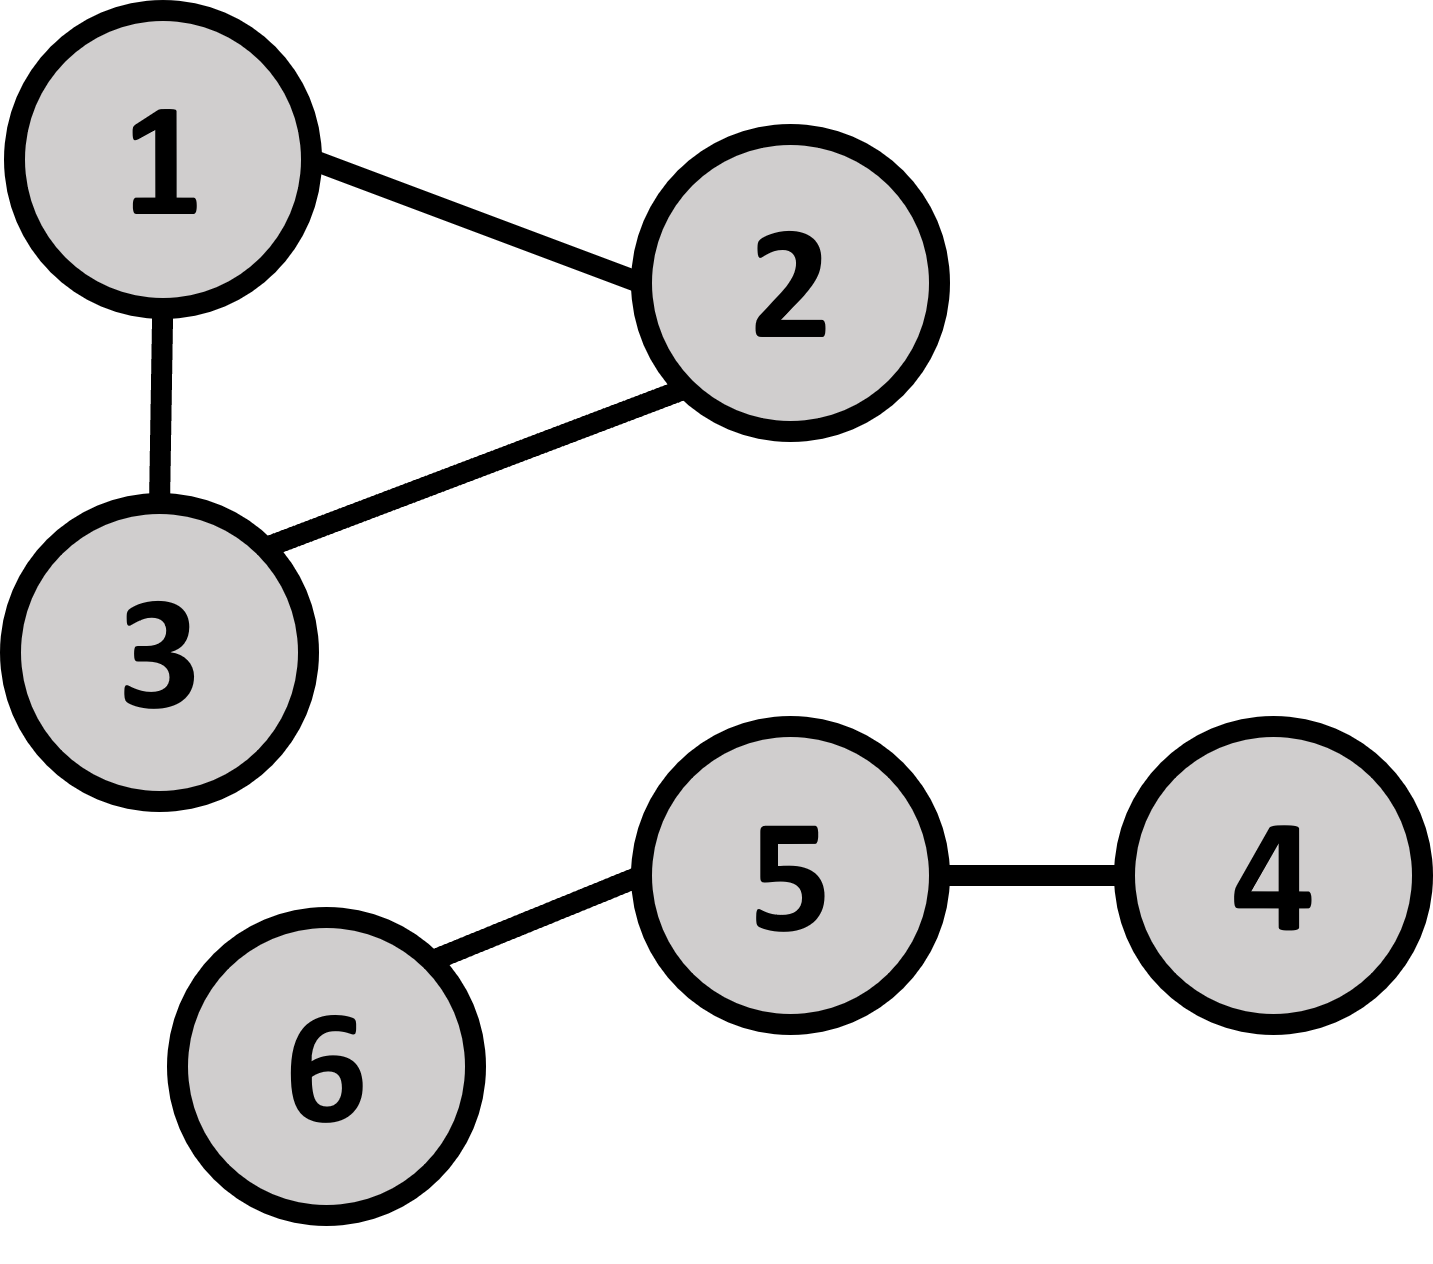
\includegraphics[scale=0.2]{grafos/islas2}
	}
\end{casebox3}

\textbf{Límites}
\begin{plimits}
	\item \(1 \leq N \leq 10^5\)
	\item \(1 \leq M \leq 2\times10^5\)
\end{plimits}

Fuente: TODO

\subsection*{Solución} 

Si descubrimos todos los vértices que se pueden alcanzar usando túneles desde \(a\), podremos saber si entre ellos esta \(b\) o no. Para esto usamos una DFS.

La idea principal es crear una DFS que regrese verdadero si puede encontrar un vértice y falso si no puede, para esto haremos que la DFS que creemos sea una función booleana que regrese la respuesta.

\begin{minipage}{\linewidth}
\begin{lstlisting}
bool buscarB(int actual, int b) {
	if (actual==b)return true;
	visitado[actual] = true;
	for (int vecino: adyacencia[actual]) {
		if (visitado[vecino] == false) {
			visitado[vecino]=true;
			if (buscarB(vecino, b)) {
				return true;
			}
		}
	}
	return false;
}

[...]

if (buscarB(a, b)) {
	cout << "SI";
} else {
	cout << "NO";
}
\end{lstlisting}
\end{minipage}

\section{Complejidad}
La complejidad de una DFS es fácil de calcular, basta con ver que cada vértice es a los más explorado una única vez; mientras que cada arista es visitada a los más dos veces, una por cada vértice que conecta.

Entonces, la complejidad total de la DFS es \(O(V+E)\). Donde \(V\) es el número de vértices y \(E\) la cantidad de aristas.

\section{Problemas clásicos}
A continuación veremos problemas clásicos de DFS, lo que querremos es que primero leas e intentes resolver los problemas. Evita leer la solución hasta haberlo intentado y se hayan acabado las ideas.

\subsection{Coloreando componentes}
Armando le gusta colorear, esta vez encontró un libro que muestra constelaciones.
El libro ilustra \(N\) estrellas conectadas con \(M\) líneas. Las estrellas están enumeradas de \(1\) a \(N\).

Una constelación es un grupo de estrellas que están conectadas entre ellas, por ejemplo la siguiente imagen muestra tres constelaciones:

\begin{center}
	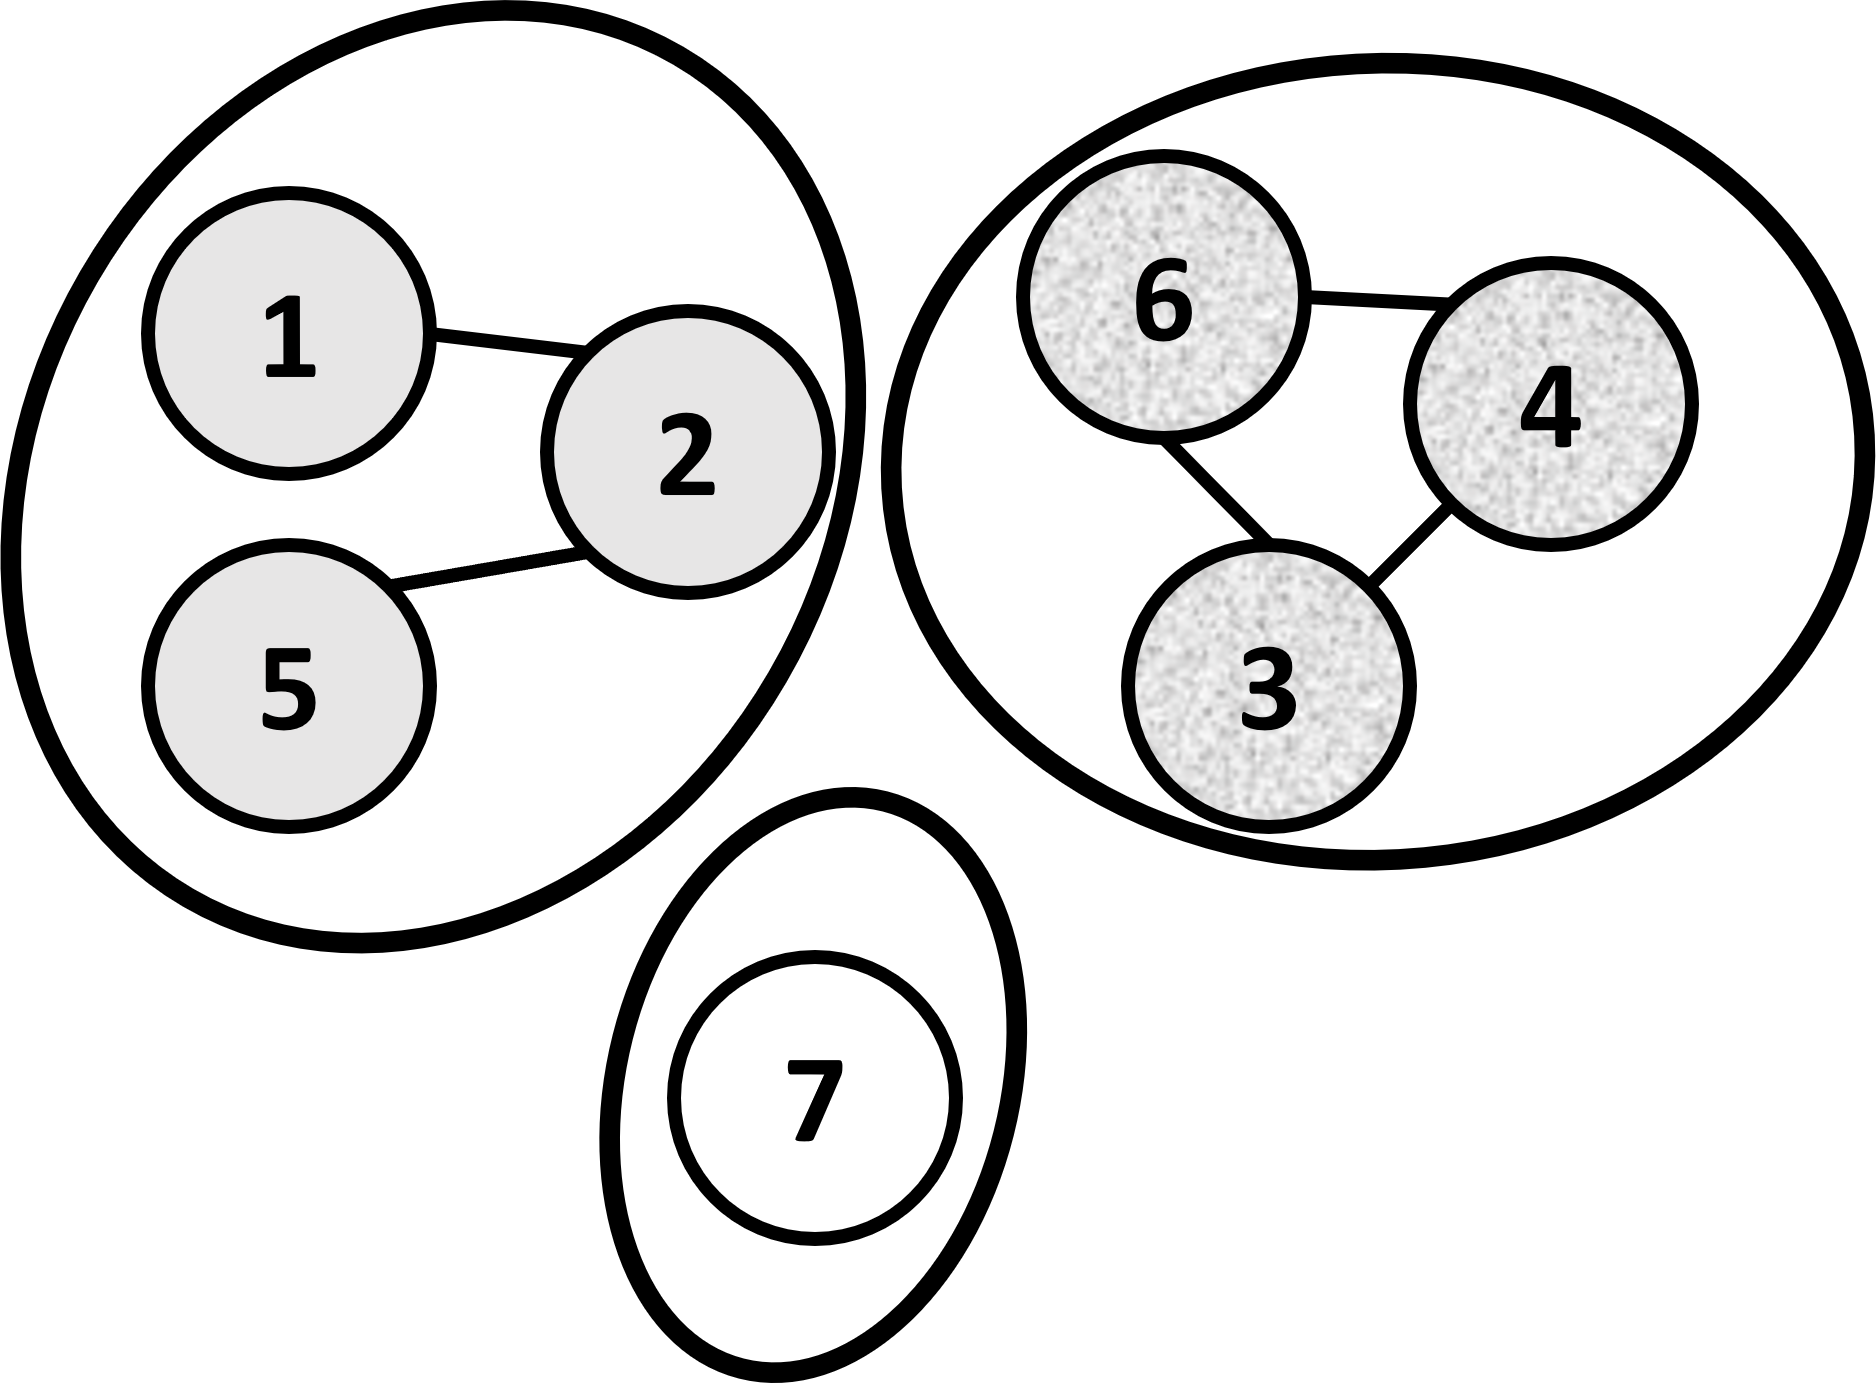
\includegraphics[scale=0.3]{grafos/constelaciones}
\end{center}

Armando quiere colorear las estrellas de forma que si dos estrellas son de la misma constelación tengan el mismo color, pero sean coloreadas diferentes si son de distintas constelaciones. Para esto el dispone de \(N\) colores enumerados \(1, 2, 3, \ldots, N\).

Dado la descripción del libro, determina el color de cada estrella que cumpla las reglas de Armando.

\textbf{Entrada}\\
La primeras dos líneas tendrán dos enteros \(N\) y \(M\) --- La cantidad de estrellas y el número de conexiones.

En las siguientes \(M\) líneas vendrán las conexiones, cada conexión será descrita por dos enteros, el número de estrellas que conecta.

\textbf{Salida}\\
Imprime \(N\) enteros, el \(i\)-ésimo entero será el color de la estrella \(i\).

Cualquier coloración válida será aceptada.

\textbf{Ejemplo}\\
\begin{casebox3}
	\ecase{
		7 5\\
		6 4\\
		4 3\\
		3 6\\
		2 5\\
		1 2
	}{1 1 2 2 1 2 3}{La imagen de ejemplo.}
\end{casebox3}

\textbf{Límites}\\
\(1\leq N \leq 10^5\)\\
\(1\leq M \leq 2\times 10^5\)

Enlace TODO:

\pagebreak

\subsubsection*{Pista}
Una pista para resolverlo es que un problema puede requerir de varias DFS.


\subsubsection*{Solución}
Una observación importante es que una constelación es un grupo de estrellas conectados ya sea de forma directa o indirecta. Este hecho significa que si iniciamos una DFS en una estrella, visitaremos todos las estrellas de la constelación.

Entonces, lo que podemos hacer es iniciar una DFS por cada constelación e ir coloreando las estrellas que vayamos visitando con un color especificado. 

Para esto, lo que haremos es un ciclo que vaya por todas las estrellas, cada que encuentre una estrella sin color, creamos una DFS que colorea su constelación.

\begin{lstlisting}
int color=0;
for (int i =0; i < N; i++) {
	if (coloreado[i]==0) {
		color++;
		dfs(i, color);
	}
}
\end{lstlisting}

\subsection{Componentes conexos}

Las constelaciones en el ejemplo anterior reciben el nombre de componente conexa, en el caso ejemplo teníamos tres componentes conexas. Entonces, una componente conexa es un conjunto de vértices más grande posible para el cual es posible viajar de uno a cualquier otro usando las aristas.

Un grafo es conexo si se puede viajar de cualquier vértice a cualquier otro usando las aristas, es decir, solo hay un componente conexo que incluye a todos los vértices.

La DFS resplandece en problemas de conectividad como lo fueron los ejemplos anteriores.

\subsection{Bipartito}
Llamamos bipartito a un grafo si se puedes separar los vértices en dos grupos de forma de que cada vértice pertenezca a exactamente un grupo y las aristas solo conecten vértices de grupos contrarios.

Por ejemplo, el siguiente grafo es bipartito:

\begin{center}
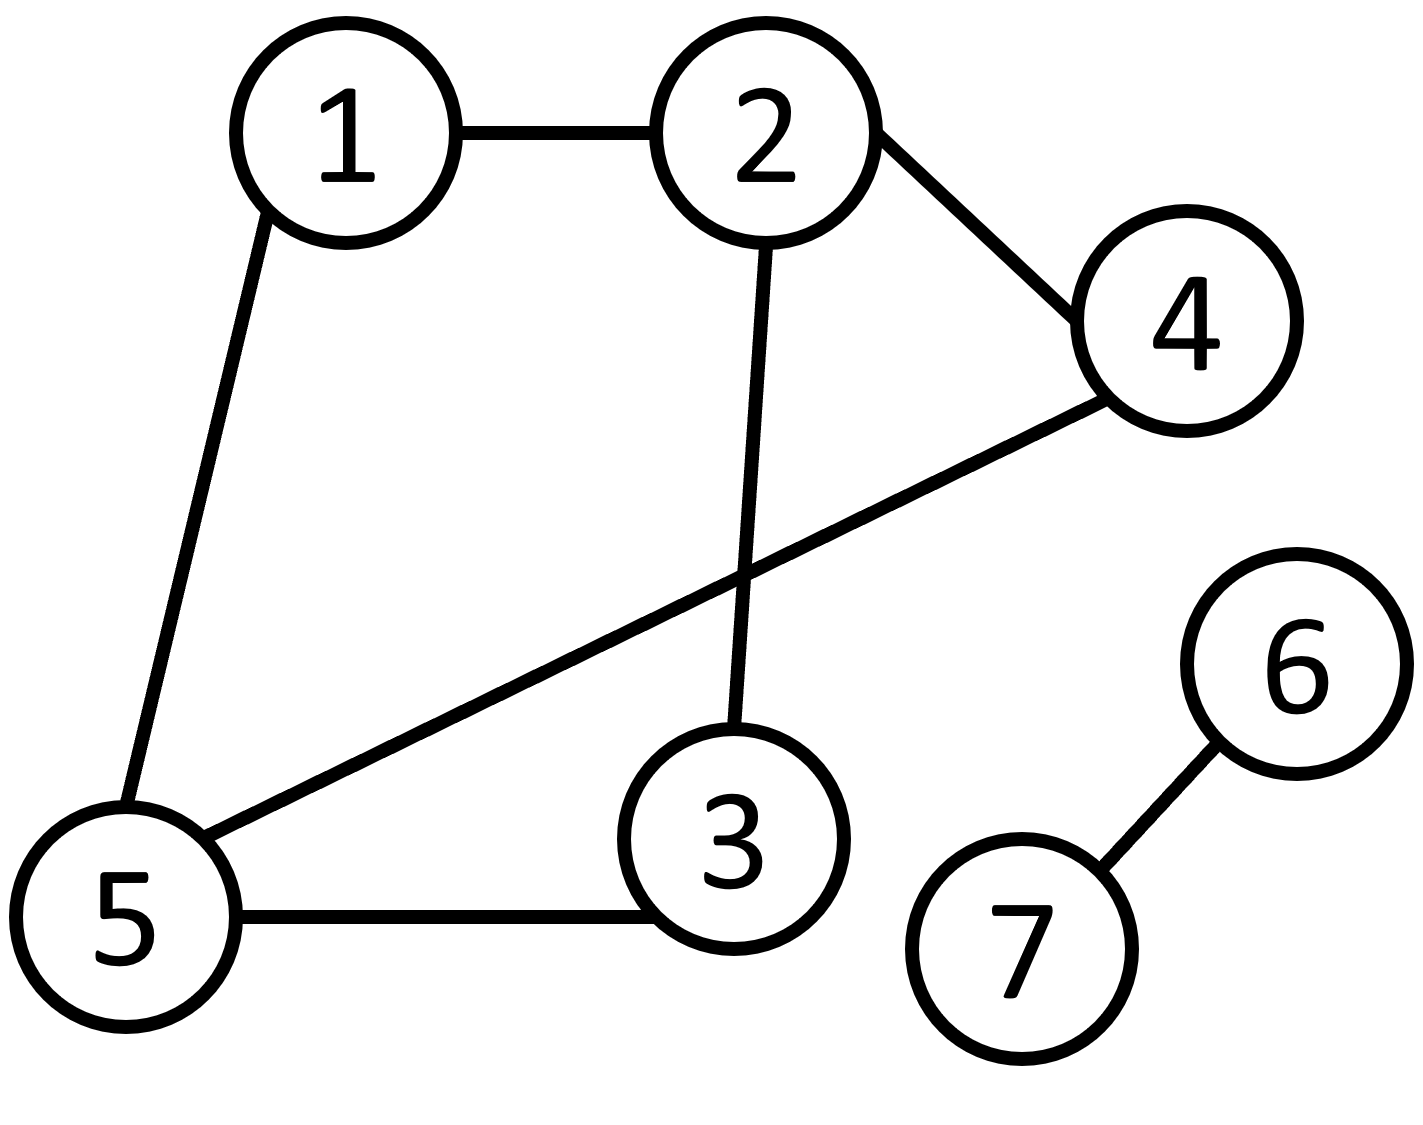
\includegraphics[scale=0.25]{grafos/bipartitoA}
\end{center}

Porque se puede separar en dos grupos \(\{2, 5, 7\}\) y \(\{1, 4, 3, 6\}\):	

\begin{center}
	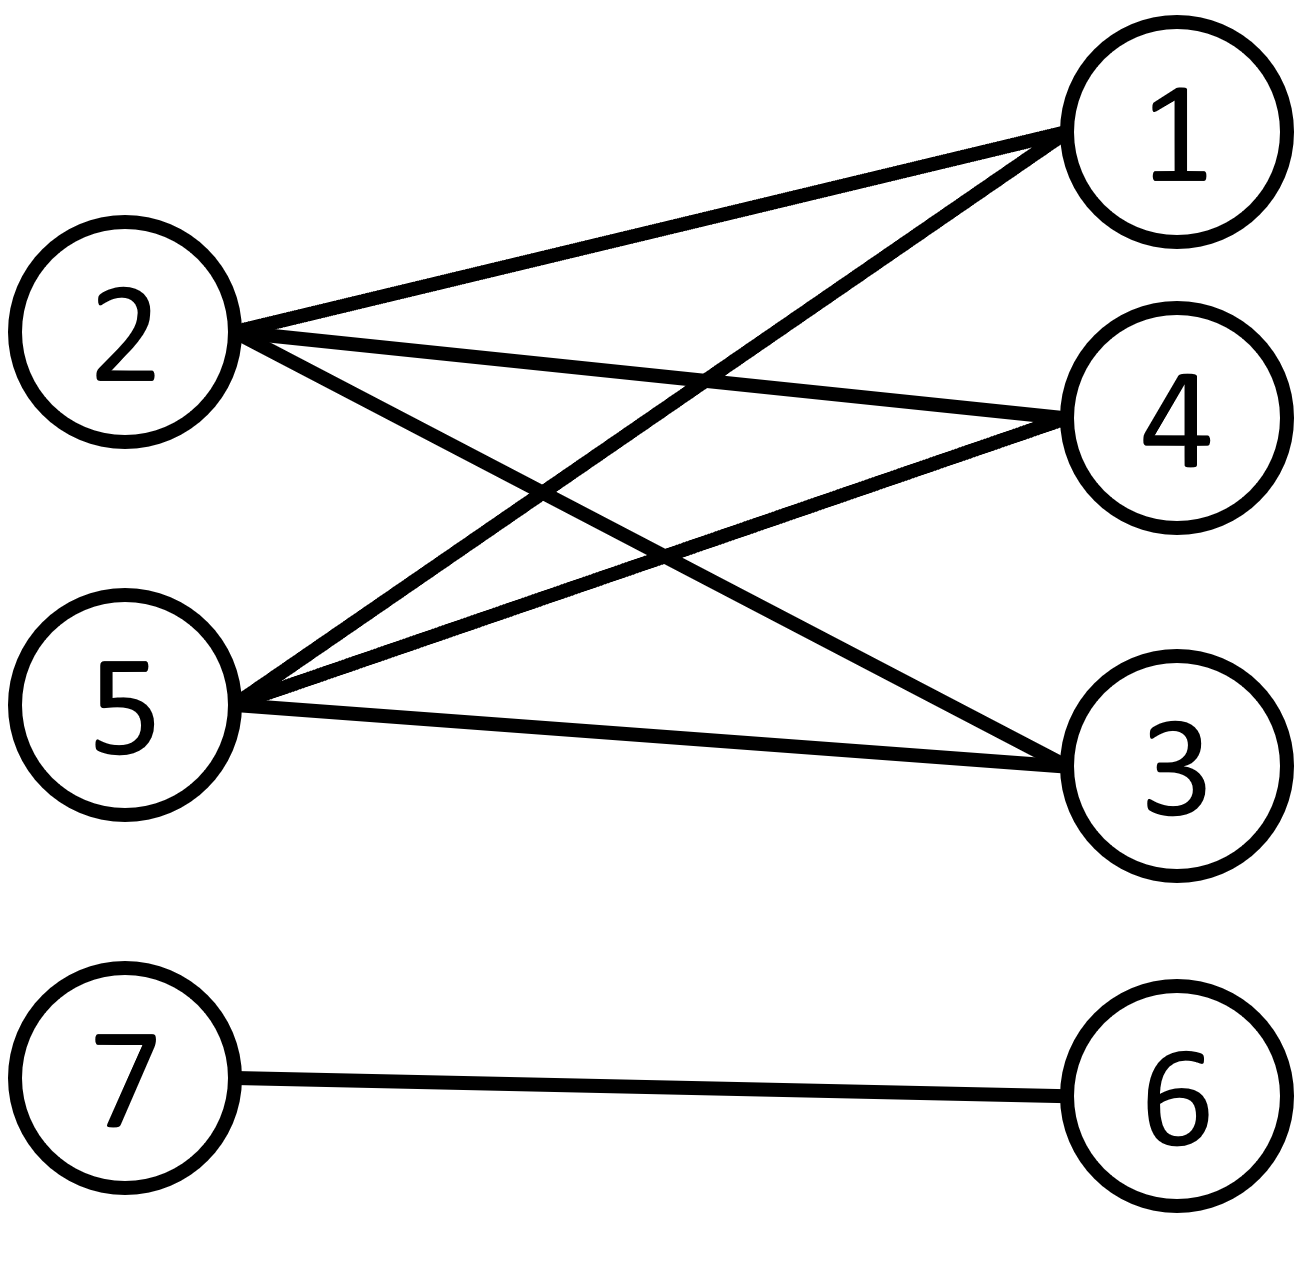
\includegraphics[scale=0.25]{grafos/bipartitoB}
\end{center}

Mientras que un grafo como el siguiente no es bipartito, no se puede separar en dos grupos con todas las aristas entre los dos grupos:

\begin{center}
	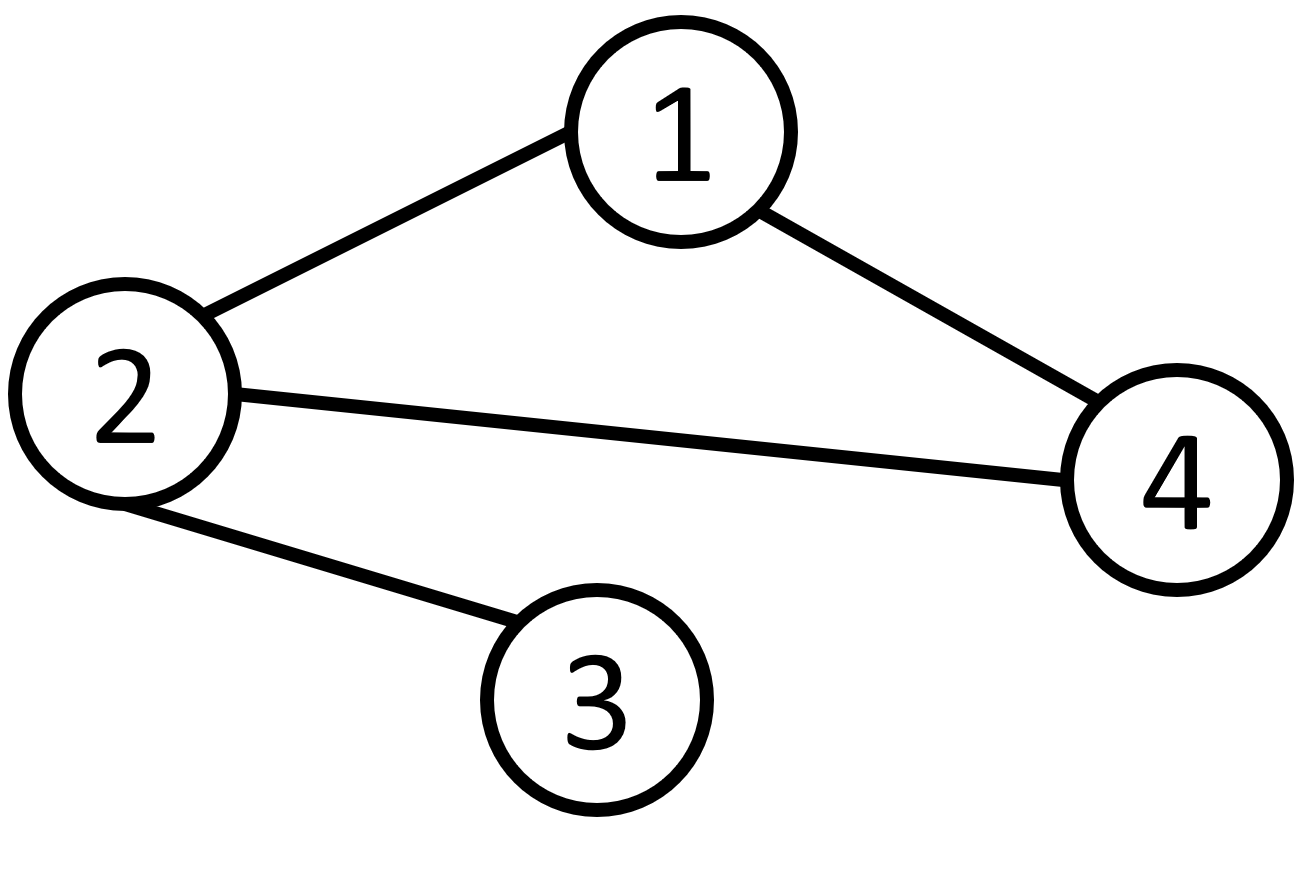
\includegraphics[scale=0.25]{grafos/nobip}
\end{center}

Dado un grafo determina si es bipartito o no.

\textbf{Entrada}\\
En la primera línea habrá dos enteros \(V\) y \(E\) --- La cantidad de vértices y aristas.

En las siguientes \(E\) líneas vendrán la descripción de las aristas.

\textbf{Salida}\\
Imprime \verb|SI| cuando el grafo sea bipartito, imprime \verb|NO| en caso contrario.

\textbf{Ejemplo}\\
\begin{casebox2}
	\scase{
		7 7\\
		1 2\\
		2 4\\
		2 3\\
		1 5\\
		5 3\\
		4 5\\
		6 7
	}{
	SI
	}
	\scase{
		4 4\\
		1 2\\
		2 4\\
		4 1\\
		2 3
	}{
	NO
	}
\end{casebox2}

\textbf{Límites}\\
\(1\leq N \leq 10^5\)\\
\(1\leq M \leq 4\times10^5\)
	

\pagebreak

\subsubsection*{Pista}
La solución sigue una idea similar al problema anterior.

\subsubsection*{Solución}
Podemos hacer una DFS que coloree el grafo con dos colores, digamos blanco y negro. 

Haremos que la DFS coloree el grafo de forma alternada tal que cada arista conecte un vértice blanco con un vértice negro. 

Evidentemente esto es lo mismo que separar los vértices en los dos grupos del grafo bipartito. Si se puede hacer esta coloración, entonces el grafo es bipartito, caso contrario no lo es.

Para esto haremos que la DFS coloree cada vértice que explore, tal que cada que se mueva una arista, alterne el color. Si en algún momento encuentras una contradicción, dos colores iguales juntos, entonces el grafo no es bipartito.


Crearemos una DFS recursiva que regrese verdadero si se puede hacer la coloración y falso en caso contrario. La DFS tiene como argumentos en cual vértice se encuentra y de que color debe ser el vértice. Alternamos el color cada que llamamos la DFS en un vecino y revisamos que en ningún momento tengamos un vecino con el mismo color.

\begin{minipage}{\linewidth}
\begin{lstlisting}
int coloreado[100050];
bool DFS(int vertice, int color) {
	int otroColor=1;
	if (color==1)
		otroColor=2;
	for (int vecino: adyacencia[vertice]) {
		if (coloreado[vecino]==0) {
			if (!DFS(vecino, otroColor)) {
				return false;
		} else if (coloreado[vecino]==color) {
			return false;
		}
	}
	return true;
}

int main() {
	[...]
	for (int i =0;i < N;i++) {
		if (coloreado[i]==0) {
			if (!DFS(i, 1)) {
				cout << "NO";
				return 0;
			}
		}
	}
	cout << "SI";
	return 0;
}
\end{lstlisting}
\end{minipage}
\chapter{Búsqueda en anchura (BFS)}
La BFS es similar a la DFS, en el sentido que explora todos los estados a los que se puede llegar a partir uno inicial.

Pero la diferencia es que esto los explora un orden diferente.

La DFS lo que hace es en un estado, explora totalmente lo que ofrezca una transición, y luego se regresa de esa exploración para ver la siguiente opción.

En cambio, la BFS lo que hace es llevar una lista de ``estados por explorar'' y procesarlos en orden. Para iniciar, revisamos todas las transiciones del estado inicial y los estados a los que nos lleven los agregamos en la lista.

Mostremos un diagrama del comportamiento de la BFS, en el diagrama los estados son representados por círculos y si han sido explorados los marcamos de gris, pero si están en la lista por explorar, los dejamos blancos. Las flechas representan las transiciones. Finalmente, los estados están enumerados en el orden que fueron alcanzados por la BFS.

\begin{center}
	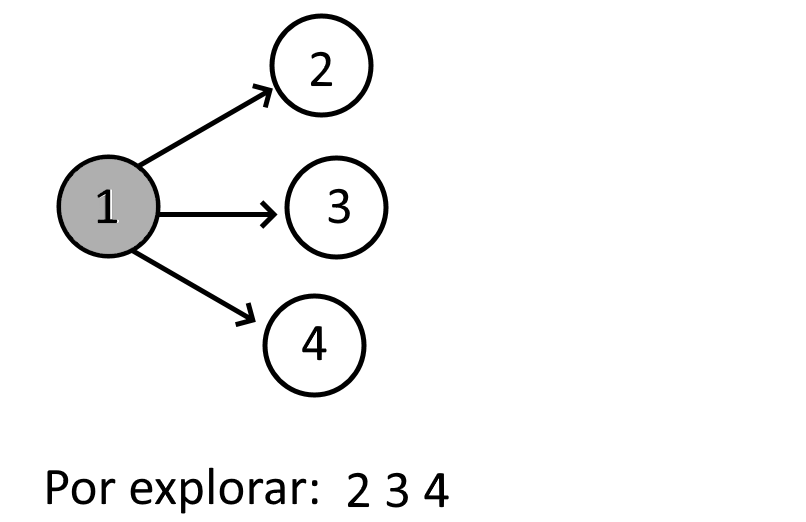
\includegraphics[scale=0.35]{bfs1}
\end{center}

Y luego para cada una de esos estados los exploramos también, es decir, expandimos las transiciones de esos estados y lo nuevo que encontremos lo ponemos en la lista de "estados por explorar". Importante: los visitamos en el orden que fueron agregados a la lista por explorar.

\begin{center}
	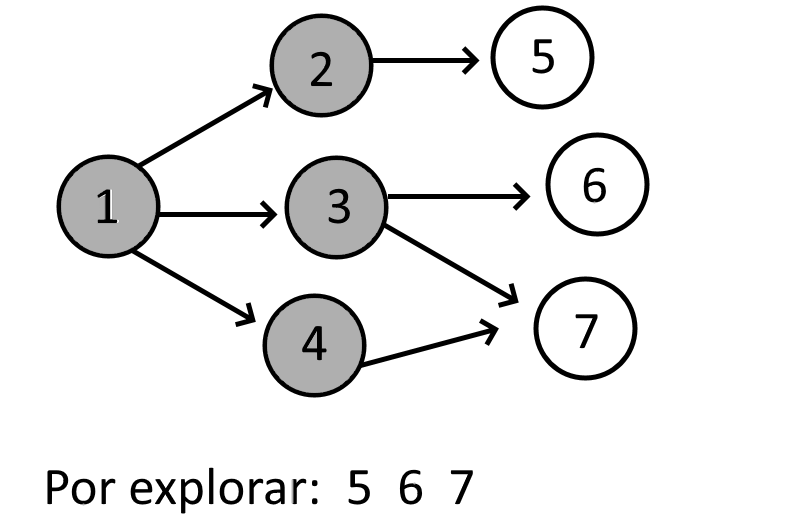
\includegraphics[scale=0.35]{bfs2}
\end{center}

De esta forma, comenzamos visitando todos los lugares alcanzables con una transición, luego dos transiciones, después tres, cuatro, cinco y  así sucesivamente.

Y precisamente, este orden en el que exploramos nos da una buena ventaja. A todo estado llegamos con la menor cantidad de transiciones posibles. Lo cual nos permite saber el mínimo número de transiciones necesarias para llegar e incluso lo podemos guardar en un arreglo o map para consultar después.

Para lograr este comportamiento, es importante ver que la lista por explorar se comporta de la siguiente forma: los estados son procesados en el mismo orden en el que entran, de forma que el primer estado en entrar a la lista es el primero en ser atendido. Este comportamiento es similar a la cola del cine, donde se atiende en el orden que llegas.

Para esto, podemos usar una estructura de datos de C++ llamada \verb|queue|, que significa cola en ingles. Si no sabes trabajar con ella, revisa la página \pageref{queue}.

Entonces, una BFS lo que hace es:

Tener una cola de la lista por explorar llamada \verb|explorar|, un arreglo de booleanos \verb|visitado| para marcar los estados que ya han sido descubiertos por la BFS y agregaremos un arreglo de enteros \verb|no_transiciones| para guardar cuantas transiciones requerimos para llegar a cada estado.

Comenzamos agregando a la lista por explorar el estado inicial con un \verb|no_transiciones| de \(0\). Luego, mientras todavía allá estados por explorar, lo procesaremos. Lo sacaremos de la pila al ya ser explorado y agregaremos a \verb|explorar| todos los estados que no hayan sido visitados alcanzables desde el estado que estamos procesando.

En código:

\begin{minipage}{\linewidth}
\begin{lstlisting}
bool visitado[];
int no_transiciones[];
void BFS(inicio) {
	queue<estados> explorar;
	cola.push(inicio);
	visitado[inicio]=true;
	no_transiciones[inicio]=0;
	while (explorar.empty()==false) {
		actual = explorar.front();
		cola.pop();
		if (actual es solucion) {
			registrar solucion actual;
			break; //opcional, si solo nos interesa una solucion
		}
		for (transiciones de actual) {
			if (!visitado[transicion]) {
				visitado[transicion]=true;
				no_transiciones[trancision]=
				no_transiciones[actual]+1;
				explorar.push(transicion);
			}
		}
	}
}
\end{lstlisting}
\end{minipage}

Como ya es de costumbre, veamos un ejemplo para entender esto.
\section*{Ejemplo: Dos operaciones}
Javier tiene una calculadora un poco peculiar. Esta muestra un número \(x\) en pantalla y tiene dos botones.

\begin{plimits}
	\item El primer botón le suma \(a\) al valor de \(x\).
	\item El segundo botón le  suma \(\frac{x}{b}\) a \(x\), pero solo puede ser presionado cuando \(x\) sea un múltiplo de \(b\).
\end{plimits}

Ahora Javier se pregunta cuantas veces debe presionar un botón para que el valor \(x\) se convierta en \(y\).

\textbf{Entrada}\\
La entrada constará de cuatro enteros: \(x\), \(y\), \(a\) y \(b\). El valor inicial de la calculadora, el valor deseado, y el valor de \(a\) y \(b\) para los botones.

\textbf{Salida}\\
Imprime un entero que sea la cantidad de pulsaciones mínima para convertir \(x\) a \(y\). Si es imposible pasar de \(x\) a \(y\) imprime \(-1\).

\textbf{Ejemplo}\\
\begin{casebox3}
	\ecase{	1 20 4 5}{6}
	{	Presiona el primer botón, ahora tienes 5.\\		
		Usa el segundo, ahora vale 6.\\
		Pulsa el primer botón, obtienes 10.\\
		Utiliza el segundo para tener 12.\\
		Usa el primer botón, obtén 16.\\
		Termina con el primero, llegamos a 20.
	}
	\ecase{	1 32 3 2}{-1}
	{	Es imposible obtener 32.
	}
\end{casebox3}

\textbf{Límites}
\begin{plimits}
	\item \(1\leq x,y,a,b \leq 10^5\)
\end{plimits}

ENLACE: TODO

\subsection*{Solución}
Entonces, en este problema nos piden la mínima cantidad de operaciones para pasar de \(x\) al valor de \(y\).

Recordemos que la BFS es perfecta para esta situaciones, pues calcula la mínima cantidad de transiciones para pasar de un estado inicial a todos los demás, incluyendo \(y\).

Para esto haremos una BFS que use de estados el número de la calculadora y de transiciones los botones. Esta explorará todas las operaciones desde \(x\) hasta llegar a \(y\).

Esto se verá:

\begin{minipage}{\linewidth}
\begin{lstlisting}
	bool visitado[100005];
	int no_transiciones[100005];
	int bfs(int x, int y, int a, int b) {
		queue<int> cola;
		cola.push(x);
		visitado[x]=true;
		no_transiciones[x]=0;		
		while (cola.empty()==false) {
			int actual=cola.front();
			cola.pop();
			if (actual==y) {
				return no_transiciones[y];
			}	
			//Primer boton
			int siguiente = actual+a;
			if (vistado[siguiente]==false){
				visitado[siguiente]=true;
				no_transiciones[siguiente]=
				no_transiciones[actual]+1;
				cola.push(siguiente);
			}
			//Segundo boton
			siguiente = actual+actual/b;
			if (actual%b == 0 && vistado[siguiente]==false){
				visitado[siguiente]=true;
				no_transiciones[siguiente]=
				no_transiciones[actual]+1;
				cola.push(siguiente);
			}
		}
		return -1;
	}
\end{lstlisting}
\end{minipage}

\section{Complejidad}
La complejidad de una BFS es sencillamente de calcular. Veamos que cada estado es colocado una sola vez dentro de la cola y por lo tanto, explorado una sola vez.

Por lo tanto, cada transición también es visitada una única vez, cuando su estado correspondiente sea visitado.

Esto provoca que la complejidad de la BFS sea \(O(V+E)\), donde \(V\) es la cantidad de estados y \(E\) es el número de transiciones.

En el ejemplo 5.1, la cantidad de estados son a lo más \(y\) y a lo más tenemos dos transiciones por estado, por lo que la complejidad es \(O(V+E)=O(y+2y)=O(y)\).\\

\section*{Problemas de práctica}
\addcontentsline{toc}{section}{Problemas de práctica}

\begin{exercise}
	\problema{Two Buttons}{\codeforceslink{520}{B}}
	Traduccion: TODO
\end{exercise}

\begin{exercise}
	\problema{Required Length}{\codeforceslink{1681}{D}}
	Traduccion: TODO
\end{exercise}

\begin{exercise}
	\problema{Camino mas corto en matriz}{TODO}
\end{exercise}

\begin{exercise}
\problema{IOI 1994 - Relojes}{\omegauplink{relojes}}
\end{exercise}

\chapter{Búsqueda binaria}

Esta técnica es una de las más poderosas e importantes en la informática. Es una forma muy eficiente de hacer búsquedas que nos permite resolver problemas antes imposibles.

Utilizada en muchas aplicaciones, nos permite resolver problemas donde una búsqueda exhaustiva tardaría miles de millones de años en menos de un segundo. Y esta impresionante herramienta ahora será tuya.

La búsqueda binaria difiere de la fuerza bruta al evitar revisar absolutamente todas las opciones del espacio de búsqueda. Si no, lo que hace es que en cada paso logra descartar la mitad del espacio de búsqueda al darse cuenta que la respuesta no está allí.

Porque en cada paso va descartando la mitad de las opciones, llega a una única opción (la respuesta si esta existe) en muy poco tiempo. Mientras que la búsqueda ehaustiva va eliminando opciones de una en una, lo cual es lento.

Comparemos un ejemplo de la búsqueda exhaustiva vs la binaria, si tuviéramos \(128\) candidatos. 
\begin{center}
	\begin{tabular}{|c|c|c|}
		\hline
		\multirow{2}{*}{\shortstack{Número\\ de pasos}} & \multicolumn{2}{c|}{Candidatos restantes} \\
		\cline{2-3}
		& Exhaustiva & Binaria \\
		\hline
		0 & 128 & 128  \\		
		\hline
		1 & 127 & 64  \\		
		\hline
		2 & 126 & 32  \\
		\hline
		3 & 125 & 16  \\
		\hline
		4 & 124 & 8  \\
		\hline
		5 & 123 & 4  \\
		\hline
		6 & 122 & 2  \\
		\hline
		7 & 121 & 1  \\
		\hline
		8 & 120 & -  \\	
		\multicolumn{3}{c}{
			\begin{LARGE}
				
				\(\cdots\)
				
			\end{LARGE} 
		}\\
		125 & 3 & - \\		
		\hline
		126 & 2 & - \\		
		\hline
		127 & 1 & - \\
		\hline
	\end{tabular}
\end{center}

Como vemos, búsqueda binaria pudo reducir los candidatos a solo uno con siete pasos, mientras que la búsqueda completa requirió de 127.

El motivo por el cuál la búsqueda binaria es tan efectiva, es que realiza \(\lceil log_2(candidatos) \rceil\) pasos \footnote{\(\lceil log_2(A) \rceil \) significa: techo del logaritmo base dos de A.\\ Recordemos que \(log_2(A)=x\) significa que \(2^x=A\).\\ Y el techo nos dice que tomemos el menor entero que sea mayor igual que el valor de adentro, por ejemplo:. \(\lceil 3.12 \rceil =4\)}. Esto es porque \(\lceil log_2 \rceil \) nos permite calcular cuantas veces podemos dividir un número entre dos hasta que sea 1.

Veamos un ejemplo que se puede resolver con búsqueda binaria.

\section*{Ejemplo: Del área al perímetro}
Javier es un granjero y esta cansado de que sus animales siempre huyan de su granja, por lo que ha decidido poner una reja al rededor de todo el terreno.

Sin embargo, Javier no sabe cuantos metros de reja va a necesitar y te ha contratado para que tu le digas esto. 

Lo que él si sabe es que el tiene forma cuadrada con lados de longitud entera, además recuerda que este mide \(A\) metros cuadrados de área.

Ayuda a Javier para que sepa cuanta reja necesita.

avier es un granjero y esta cansado de que sus animales siempre huyan de su granja, por lo que ha decidido poner una reja al rededor de todo el terreno.

Sin embargo, Javier no sabe cuantos metros de reja va a necesitar y te ha contratado para que tu le digas esto. 

Lo que él si sabe es que el tiene forma cuadrada con lados de longitud entera, además recuerda que este mide \(A\) metros cuadrados de área.

Ayuda a Javier para que sepa cuanta reja necesita.

\textbf{Entrada}\\
Un entero \(A\), el tamaño del terreno en metros cuadrados.

\textbf{Salida}\\
Un entero indicando cuantos metros de reja necesita para rodear todo el terreno. 

\textbf{Ejemplos}\\
\begin{casebox2}
	\scase{36}{24}
	\scase{100}{40}
	\scase{1}{4}
\end{casebox2}

\textbf{Límites}
\begin{plimits}
	\item \(1\leq A \leq 10^{18}\)
\end{plimits}

\textbf{Subtareas}
\begin{plimits}
	\item (35 pts) \(1\leq A \leq 10^9\)
	\item (65 pts) Sin restricciones adicionales
\end{plimits}

ENLACE: TODO

\subsection*{Solución}
Como siempre, antes de leer la solución te invitamos a que intentes el problema.

En este problema nos piden de que dado el área de un cuadrado, imprimamos el perímetro. Por esto, recordemos las fórmulas del cuadrado.
\[Per\acute{i}metro=4\times Lado \]
\[\acute{A}rea=Lado\times Lado \]

Entonces, si encontramos el lado que nos de el área de entrada, podremos encontrar el perímetro.

Para este problema vamos a ver dos estrategias para resolverlo, la de búsqueda lineal y la binaria.

Comencemos con la que ya deberíamos estar familiarizada, usemos búsqueda lineal.
\subsection*{Búsqueda lineal}
Entonces, buscaremos el entero \(L\) de entre todos los posibles, que cumpla que \(A=4\times L\). Para esto, podremos ir probando del \(1\) en adelante hasta encontrar el que cumpla.

\begin{lstlisting}
	long long L=1;
	while (L*L != A) {
		L++;
	}
\end{lstlisting}

Esto itera por todos los enteros del \(1\) a la respuesta que es \(\sqrt{A}\). Por lo tanto, su complejidad es \(O(\sqrt{A})\). Lo cual es suficiente para la subtarea de 35 puntos, pero no para el límite completo de \(10^{18}\).

\subsection*{Búsqueda binaria}
Ahora resolvamos el problema utilizando búsqueda binaria.

Definamos nuestro espacio de búsqueda, ¿cuáles valores puede ser \(L\)? y si lo pensamos puede ser desde \(1\) hasta \(10^9\). Porque \(10^9\times 10^9=10^{18}\) y de los límites sabemos que \(1\leq A\leq 10^{18}\).

Entonces queremos encontrar la respuesta que esta entre \(1\) y \(10^9\), hagamos una función que logre esto llamada buscar que reciba el rango de donde esta la respuesta.

\begin{lstlisting}
	//Encuentra L tal que L*L=A, sabiendo que a<=L<=b.
	long long buscar(long long a, long long b, long long A);
\end{lstlisting}

Ahora tenemos \(10^9\) candidatos donde encontrar la respuesta y queremos reducirlo a la mitad. 

Para esto podemos ver que sucede con \(5\times10^8\). 

Si resulta que \((5\times10^8)\times(5\times10^8) <A\), entonces sabemos que cualquier valor menor igual que \(5 \times 10^8\) no funcionará porque es demasiado pequeño. Por lo tanto la respuesta debe estar entre \(5\times 10^8 +1\) y \(10^9\) y los candidatos se redujeron a la mitad.

Pero si en vez sucede que \((5\times10^8)\times(5\times10^8) >=A\), entonces sabremos que cualquier valor más grande que \(5\times 10^8\) nos dará valores más grandes que \(A\) y por lo tanto la respuesta no estará allí. Ahora nuestros candidatos son los números entre \(1\) y \(5\times 10^8\), reduciendo los valores que podrían ser la respuesta a la mitad.

Y de hecho, si en general, la respuesta esta entre \(a\) y \(b\), nos convendrá preguntar por el punto medio \((a+b)/2\), que nos reducirá el espacio a la mitad.

Una vez que redujimos el rango de la búsqueda, tendremos que encontrar la respuesta en ese nuevo rango, y para esto podemos hacer recursión.

De forma que ahora tenemos:

\begin{minipage}{\linewidth}	
\begin{lstlisting}
long long buscar(long long a, long long b, long long A) {
	long long m =(a+b)/2;
	if (m*m < A) {
		return buscar(m+1, b, A);
	} else {
		return buscar(a, m, A);
	}
} 
\end{lstlisting}

\end{minipage}


Ahora, lo que le falta a esa recursión es una condición de paro, saber cuando ya termino y encontramos la respuesta.

Podremos ver que habremos encontrado la respuesta cuando ya estemos seguros de cual es esta. Y esto sucede cuando nuestro rango solo incluye un valor, es decir, cuando \(a==b\) se cumpla.

\begin{minipage}{\textwidth}
\begin{lstlisting}
long long buscar(long lonng a, long long b, long long A) {
	if (a==b)
		return a;
	long long m=(a+b)/2;
	if (m*m<A) {
		return buscar(m+1, b, A);
	} else {
		return buscar(a, m, A);
	}
}
\end{lstlisting}
\end{minipage}
Y con esto, tenemos que \verb|L=buscar(1, 1000000000, A)|.

Ahora, la complejidad de esto es \(O(log(\sqrt{A}))\), lo cual corre perfectamente para \(10^{18}\).

\textbf{Nota:} En este problemas también se pudo haber usado \lstinline|L=sqrt(A)| con la librería \verb|<math.h>| que calcula el valor rápidamente, pero se uso búsqueda binaria para ejemplificar.

También puede ser escrita de forma iterativa de la siguiente manera:

\begin{minipage}{\textwidth}
	\begin{lstlisting}
long long buscar(long lonng a, long long b, long long A) {
	while (a!=b) {
		long long m=(a+b)/2;
		if (m*m < A) {
			a=m+1;
		} else {
			b=m;
		}
	}
	return a;
}
	\end{lstlisting}
\end{minipage}

\section*{Ejemplo: Buscar en un arreglo}
Se te da un arreglo \(A\) de \(N\) enteros diferentes. El arreglo estará en orden creciente, es decir, \(A[i] < A[i+1]\).

Deberás responder \(T\) preguntas:

Cada pregunta consistirá de un entero \(q_i\) y tu deberás imprimir el índice del valor \(q_i\) o \(-1\) si este valor no existe.
\textbf{Entrada}\\
El enteros \(N\).

En la siguiente línea: \(N\) enteros separados, los valores del arreglo \(A\).

En la siguiente línea recibirás el entero \(T\).

En las siguientes \(T\) líneas recibirás los valores de cada pregunta.

\textbf{Salida}\\
Imprime la respuesta cada pregunta en una línea en el mismo orden que el de lectura.

\textbf{Ejemplo}\\
\begin{casebox2}
	\scase{
		7\\
		2 5 6 7 8 9 10\\
		5\\
		2\\
		6\\
		4\\
		10\\
		5\\
	}
	{
		0\\
		2\\
		-1\\
		6\\
		1		
	}
\end{casebox2}

\textbf{Límites}
\begin{plimits}
	\item \(1\leq N,T \leq 10^5 \)
	\item \(1\leq A[i], q_i \leq 10^9 \)
\end{plimits}

Enlace: TODO

\subsection*{Solución}
Esta ocasión nos piden encontrar el indice de un valor en un arreglo ordenado. Ya hemos visto como hacerlo con búsqueda lineal:

\begin{lstlisting}
	int indice(int q) {
		for (int i =0; i < N;i++) 
		if (A[i]==q)
		return i;
		return -1;
	}
\end{lstlisting}

Sin embargo, esto no corre en tiempo ya que la complejidad es \(O(N)\) por pregunta, siendo en total \(O(TN)\) y como \(TN=10^{10}\), obtendremos TLE.

Pero veamos que podemos usar búsqueda binaria. ya que al preguntar por una posición de en medio y discernir si tenemos que buscar adelante o atrás.

\begin{lstlisting}
	int binaria(int a, int b, int q) {
		if (a>b)
		return -1;
		int m =(a+b)/2;
		if (A[m]==q)
		return m;
		if (A[m]<q) {
			return binaria(m+1, b, q);
		} else {
			return binaria(a, m-1, q);
		}		
	}
	int indice(int q) {
		return binaria(0, N-1, q);
	}
\end{lstlisting}

La nueva complejidad ahora es \(O(logN)\) por pregunta, en total\\ \(O(TlogN)\).

\section{Dificultades}
Ya vimos que la búsqueda binaria tiene una ventaja enorme sobre la búsqueda lineal ya que resuelve el problema en un tiempo mucho menor.

Pero tristemente, no siempre es posible aplicar la búsqueda binaria. Hay veces en las que no podemos descartar fácilmente la mitad de los candidatos.

Un caso donde puede suceder sería en el ejemplo anterior si el arreglo no estuviese ordenado. En ese caso no podríamos hacer el truco de solo revisar adelante si \(A[m]<q\) ya que no nos da suficiente información esa pregunta para eliminar todos los valores de \(0\) a \(m\).

Por supuesto, el problema anterior tiene corrección para que la búsqueda binaria siga funcionando y muchas veces esto es parte del problema, ¿cómo hago la binaria aquí? Pero hay otras veces que es imposible, o al menos, más allá de los conocimientos actuales.

En esos casos, no quedará de otra más que hacer búsqueda completa o usar una técnica diferente a búsqueda.

Otro ejemplo donde la búsqueda binaria no se puede utilizar es en encontrar el primer divisor que no sea 1 de un entero. Es difícil descartar la mitad de candidatos en una sola operación. 




\section{Función de validación}
\markright{FUNCIÓN DE VALIDACIÓN}
Igual que en búsqueda lineal podíamos agregar funciones más complicadas a la hora de buscar la respuesta, lo mismo sucede en búsqueda binaria. A veces requeriremos de más código que una simple comparación para saber en cual mitad esta la respuesta.

Veamos unos ejemplos.


\subsection*{Ejemplo: Bicicleta de Karel II}
Karel ha comprado una bicicleta eléctrica con la que planea completar un recorrido. El recorrido se puede ver como \(N\) colinas en línea recta tal que la \(i\)-ésima colina tiene altura \(h_i\). Karel comienza en la colina hasta la izquierda y quiere terminar en la ultima colina de hasta la derecha.

Cuando Karel sube un metro gasta \(1\) unidad de energía, mientras que bajar un metro recupera \(1\) unidad de altura. Si Karel en algún momento necesita subir, pero su batería tiene 0 de energía, Karel se quedará atorado y no terminará el recorrido.

Por suerte al inicio hay una estación de recarga donde Karel puede recargar su bicicleta. Como nota, la batería tiene capacidad \(R\) y jamás podrá almacena más energía que \(R\).

Actualmente Karel tiene \(0\) de energía, Determina cuál es la menor cantidad de energía que es necesaria recargar al inicio para completar el recorrido. O determina si es imposible hacer el recorrido con la bicicleta de Karel.

\subsubsection*{Entrada}
La primera línea tiene dos enteros, el valor de \(N\) y \(R\).

En la siguiente línea vienen \(N\), enteros separados por espacios, siendo la altura de las colinas de izquierda a derecha. Recuerda que Karel comienza en la primera colina y quiera terminar en la última.
\subsubsection*{Salida}
Un entero, representando la menor cantidad de energía necesaria para completar el recorrido. Si Karel no puede completar el recorrido, imprime \(-1\).

\subsubsection*{Casos ejemplo}
\begin{casebox3}	
	\ecase{
		6 8\\
		4 6 3 5 7 
	}
	{3}
	{
		Karel inicia con 3 de energía, moverse de   \\
		la primera a la segunda colina le toma 2,  \\
		ahora tiene 1.\\
		Luego avanza y se recarga 3,\\
		ahora tiene 4.\\
		Después continua y se consume 2, ahora tiene 2. \\
		Vuelve a avanzar quedándose con 0 de energía. \\		
		Pero luego avanza y se recarga a 5. \\
		Finalmente avanza para termina con 5. \\
	}
	\ecase{
		5 6\\
		1 10 1 2 0
	}
	{-1}
	{}
	\hline
\end{casebox3}	

\subsubsection*{Límites}
\begin{plimits}
	\item \(2\leq N, R \leq 10^5\)
	\item \(0\leq h_i\leq 10^9\)
\end{plimits}

Fuente: OMIS online 2022.\\
\footnotesize{(\omegauplink{Bicicleta-de-Karel})}

\subsection*{Solución}
Este problema 1.6 de búsqueda lineal con validación en la página \pageref{bicicleta}, si no sabes resolverlo con búsqueda lineal para los límites de allí, primero descubre esa solución.

Esta vez, los límites son más estrictos, de forma que la solución estándar con búsqueda lineal no funciona, pero veamos cual es porque nos será útil.
\\

La respuesta siempre estará entre \(0\)  y\(R\). La búsqueda lineal funciona de la siguiente manera.
\begin{lstlisting}
	int respuesta=-1;
	for (int e=0; e<=R; e++) {
		if (funciona(e)) {
			respuesta=e;
			break;
		}
	}
\end{lstlisting}

Y la función \verb|bool funciona(int e)| te regresa verdadero si Karel puede completar el recorrido comenzando con \(e\) de energía.

Esta función simplemente simula el recorrido para ver si Karel se atora en algún momento. Se ve de la siguiente forma:

\begin{lstlisting}
	bool funciona(int e) {
		for (int i = 1; i <N; i++){
			e-=A[i]-A[i-1];
			if (e > R) 
			e=R; //Limita la energia
			if (e < 0)
			return false;			
		}
		return true;
	}
\end{lstlisting}

La función \verb|funciona()| tiene una complejidad de \(O(N)\) y como es llamada en \(R\) valores, la complejidad total es \(O(RN)\).

Pero ahora veamos dos hechos importantes:
\begin{itemize}
	\item Si funciona(m) cumple, también lo hará cualquier valor mayor que \(m\).
	\item Si funciona(m) falla, también lo hará cualquier valor menor que \(m\).
\end{itemize}

Es decir, el rango de búsqueda se ve de la siguiente forma:

\begin{center}
	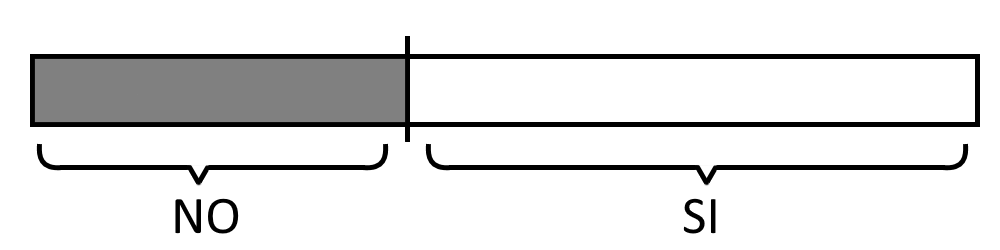
\includegraphics[scale=0.3]{binprop}
\end{center}

Esto hace que podamos hacer búsqueda binaria para encontrar el primer SI.

El código se verá como:

\begin{lstlisting}
	int a=0,b=R;
	while(a!=b) {
		int m=(a+b)/2;
		if (funciona(m)) {
			b=m;
		} else {
			a=m+1;
		}
	}
	int respuesta=-1;
	if (funciona(a))
	respuesta=a;
\end{lstlisting}

\section{Complejidad}

La complejidad de la búsqueda binaria es entonces \(O(logN)\), donde \(N\) es el tamaño del espacio de búsqueda porque \(logN\) nos dice cuantas veces \(N\) puede ser dividido entre dos. 

Pero también, en cada paso de la búsqueda podemos usar una llamada de validación. En el ejemplo anterior estamos llamando a \verb|funciona()| que tiene complejidad \(O(N)\), por lo tanto, la complejidad total es \(O(NlogR)\).

Es decir, la complejidad de una búsqueda binaria es \(O(busqueda \times validacion)\) que es igual a \(O(logN \times validacion)\).


\section*{Problemas de práctica}
\addcontentsline{toc}{section}{Problemas de práctica}

\begin{exercise}
	\problema[barcos-turisticos]{Barcos turísticos}{\omegauplink{Barcos-turisticos}}
\end{exercise}

\begin{exercise}
	\problema{Subcadena de suma K}{TODO}
\end{exercise}
\section{Búsqueda en los reales}
\markright{BÚSQUEDA EN LOS REALES}
Hay veces en la que no estamos buscando un valor entero, si no en vez querremos encontrar un valor real a cierta precisión.

El problema dirá algo por el estilo de: imprime la respuesta con precisión de \(10^{-6}\), esto quiere decir que tu respuesta no debe estar alejada de la solución por más de \(10^{-6}\).

Para estos problemas debes cambiar la condición de paro de \(a==b\), por \(b-a < precision\). Aunque en realidad, recomiendo poner una precisión un poco más ajustada ya que no tiende a aumentar mucho el costo y permite una programación más relajada.

De forma que ahora la binaria se verá como:

\begin{lstlisting}
double a =0, b=1e9;
double epsilon = 1e-8;
while(b-a>= epsilon) {
	double m = (a+b)/2;
	if (funciona(m)) {
		b=m;
	} else {
		a=m;
	}
}
\end{lstlisting}

\section{Ejemplo: Raíz cuadrada real}
Calcula la raíz cuadrada de un número A con precisión absoluta de \(10^{-4}\).

\textbf{Ejemplo}\\
\begin{casebox2}
	\scase{10}{3.1622}
	\scase{16}{4.0000}
\end{casebox2}

\textbf{Límites}
\begin{plimits}
	\item \(1\leq A \leq 10^9\)
\end{plimits}

\subsection*{Solución}
Usamos las mismas observaciones que usamos para el ejemplo ``De área a perímetro", pero esta vez lo haremos con \lstinline|double| y nos detenemos basados en una precisión.
\begin{lstlisting}
	double raiz(double A) {
		double a=0, b=A;
		while (b-a >= 1e-5) {
			double m=(a+b)/2;
			if (m*m < A) {
				a=m;
			} else {
				b=m;
			}
		}
		return a;
	}
\end{lstlisting}

\subsection{Complejidad}
La complejidad de este procedimiento sigue siendo \(O(log(Espacio))\), pero ahora debemos encontrar el tamaño del espacio de búsqueda. 

Con un poco de matemáticas veremos que es \(E=\frac{R-L}{precision}\), en el caso de ejemplo la precisión es pues: \(\frac{A}{10^{-4}}\), aunque nosotros usamos una precisión de \(10^{-5}\), por lo que es \(\frac{A}{10^{-5}}\).

Por lo tanto, la complejidad del ejemplo anterior es:
\[O(logE)\]
\[ = O(log\frac{A}{10^{-5}})\]
\[ = O(log(A)-log({10^{-5}}))\]
\[ = O(log(A)+log({10^{5}}))\]

Entonces, poner una precisión de \(10^-5\) solo nos aumenta un costo de \(log(10^5)=16.6\), o en otras palabras, 17 preguntas extra.

\section*{Problemas de práctica}
\addcontentsline{toc}{section}{Problemas de práctica}

\begin{exercise}
	\problema{Carreras de la Formula \(\pi\) }{TODO}
\end{exercise}

\begin{exercise}
	\problema{Planetas}{\omegauplink{planetas}}
\end{exercise}

\begin{exercise}
\problema{Carretera}{\omegauplink{carretera}}
\end{exercise}
\section*{Problemas de práctica}
\addcontentsline{toc}{section}{Problemas de práctica}
\markright{Problemas de práctica}

\begin{exercise}
	\problema{Contando LaserTag justos}{TODO}
\end{exercise}

\begin{exercise}
	\problema[torre-I]{Subiendo la torre}{TODO}
\end{exercise}

\begin{exercise}
	\problema{Mapas}{\omegauplink{OMI-2020-Mapas}}
\end{exercise}

\begin{exercise}
	\problema[problemas/frecuencia-de-k]{TODO Frecuencia de K}{\omegauplink{frecuencia-de-k}}
\end{exercise}

\begin{exercise}
	\problema[problemas/multiplos-de-cinco]{TODO Multiplos de cinco}{\omegauplink{multiplos-cinco}}
\end{exercise}

\begin{exercise}
	\problema[problemas/divisores]{TODO: Divisores del entero}{\omegauplink{divisores-entero}}
\end{exercise}

\begin{exercise}
	\problema[problemas/suma-de-digitos]{A la suma de digitos}{\omegauplink{m-suma-digitos}}
\end{exercise}

\begin{exercise}
	\problema[problemas/escalera-de-fer]{Escalera de fer}{TODO}
\end{exercise}

\begin{exercise}
	\problema[problemas/bicicleta-de-karel]{Bicicleta de Karel I}{\omegauplink{bicicleta-de-karel-i}}
\end{exercise}

\begin{exercise}
	\problema[problemas/contar-capicuas]{Contar capicúas}{\omegauplink{Contar-capicuas}}
\end{exercise}

\begin{exercise}
	\problema[problemas/cuenta-primos]{Cuenta primos}{\omegauplink{Cuenta-primos}}
\end{exercise}

\begin{exercise}
	\problema[inversiones-arreglo]{TODO Inversiones en el arreglo}{\omegauplink{inversiones-arreglo}}
\end{exercise}

\begin{exercise}
	\problema[contar-sumas-pares]{TODO Puntuación de la ferretería}{\omegauplink{contar-sumas-pares}}
\end{exercise}

\begin{exercise}
	\problema[algofashion-fibo]{TODO Números de moda}{\omegauplink{moda-fibonacci}}
\end{exercise}

\begin{exercise}
	\problema[terreno-valioso]{TODO Terreno más valios}{\omegauplink{TODO terreno-valioso}}
\end{exercise}

\begin{exercise}
	\problema[suma-modulo-k]{TODO Suma modular}{\omegauplink{TODO suma-modulo-k}}
\end{exercise}

\begin{exercise}
	\problema[warel-roba-diamantes]{Warel roba diamantes}{\omegauplink{warel-roba-diamantes}}
\end{exercise}

\begin{exercise}
	\problema[imprime-binarios]{Imprime números binarios}{\omegauplink{Imprime-binario}}
\end{exercise}

\begin{exercise}
	\problema[reverse-matrix]{Invirtiendo una matriz}{\omegauplink{TODO reverse-matrix}}
\end{exercise}


\part{Matemáticas olímpicas}

\part{STL y estructuras de datos}

\part{Grafos}

\part{Técnicas de resolución de problemas}

\part{Problemas no estándar}

\backmatter


\end{document}